\renewcommand{\nomducours}{\nomcoursquatre}
\renewcommand{\chapterlabel}{chap_quatre}
\renewcommand{\sousnomducours}{\sousnomcoursquatre}
\renewcommand{\contentsummaryducours}{\contentsummarycoursquatre}

\chapter{\nomducours}
\thispagestyle{empty}
\label{\chapterlabel}

\begin{tetedechapitre}[\contentsummaryducours]
	Au cours des chapitres~\deux et~\trois nous avons appris à quantifier les transferts d’énergie, mais nous ne pouvons le faire que si nous connaissons les valeurs de $u$ ou de $h$, propriétés qu’il est impossible de mesurer directement en pratique.
	
Ce \coursquatre se propose de répondre à deux questions :
\begin{itemize}
	\item Comment peut-on décrire le comportement de l’air lorsqu’il est chauffé ou comprimé ?
	\item Comment peut-on prévoir les valeurs de $u$ et de $h$ lorsqu’on utilise de l’air ?
\end{itemize}
Ce chapitre est incompatible avec le \courscinq, où nous devrons oublier tout ce qui est appris ici.
\par
\end{tetedechapitre}

\section{Définition}

	\subsection{Le manomètre comme thermomètre}
	\label{ch_le_manomètre_comme_thermomètre}

		Commençons par le plus important :

		\begin{trucimportant}
			Le gaz parfait est un \textit{modèle mathématique},\linebreak
			permettant de prédire la température d’un gaz en fonction de sa pression.
		\end{trucimportant}

		Le modèle du gaz parfait définit de lui-même une échelle de température. On propose de mesurer très simplement la température absolue $T$ avec un manomètre, en stipulant qu’elle est directement proportionnelle à la pression $p$ et inversement proportionnelle à la masse volumique $\rho$.

		On peut ainsi dire que le gaz parfait ne décrit pas la réalité des choses, que ce n’est pas un principe physique, mais bien seulement un modèle simplifié du comportement des gaz. Sa plage de validité est limitée et floue.



		\subsection{Définition : l’équation d’état}

				\thermoquotebegin{O}
			Le changement de température occasioné dans les gaz par le changement de volume peut être regardé comme l’un des faits les plus importans de la physique, à cause des nombreuses conséquences qu’il entraîne, et en même temps comme l’un des plus difficiles à éclaircir et à mesurer par des expériences décisives. Il semble présenter dans plusieurs circonstances des anomalies singulières.\nolinebreak\makebox(18,5){\color{gray}\scalebox{2}{»}}\par\vspace{-0.3cm}\begin{flushright}Sadi Carnot, 1824~\cite{carnot1824}\end{flushright}
		\makebox(18,5){\color{gray}\scalebox{2}{«}}
		M. S. Carnot, évitant l’emploi de l’analyse mathématique, arrive par une série de raisonnemens délicats et difficiles à saisir, à des résultats qui se déduisent sans peine d’une loi plus générale, que je vais chercher à établir.
		\thermoquoteend{Émile Clapeyron, 1834~\cite{clapeyron1834}}{}
		Nous appellerons \vocab{gaz parfait} (ou \vocab{gaz idéal}) un fluide à l’état gazeux dont le multiple de la pression et du volume, $p v$, reste proportionnel à sa température. La constante de proportionnalité est nommée \vocab{constante du gaz}, et notée $R$ ; elle dépend de la nature du~gaz.
		\begin{equation}
			p v = R T
			\label{eq_pv=RT}
		\end{equation}
		\begin{equationterms}
			\item par définition pour un gaz parfait,
			\item où \tab $p$ \tab est la pression (\si{\pascal}),
			\item 	\tab $v$ \tab le volume spécifique (\si{\metre\cubed\per\kilogram}),
			\item 	\tab $T$ \tab la température (\si{\kelvin}),
			\item et \tab $R$ \tab la constante du gaz considéré (\si{\joule\per\kelvin\per\kilogram}).
		\end{equationterms}

		L’\cref{eq_pv=RT} est nommée \vocab{équation d’état des gaz parfaits}. Elle peut également être exprimée en fonction de la masse :
		\begin{equation}
			p V = m R T
			\label{eq_pV=mRT}
		\end{equation}
		\begin{equationterms}
			\item où \tab $V$ \tab est le volume (\si{\metre\cubed}),
			\item et \tab $m$ \tab la masse de gaz considérée (\si{\kilogram}).
		\end{equationterms}
		
		Il est aussi possible d’exprimer l’\cref{eq_pV=mRT} en fonction de la quantité de matière en \si{moles}.\footnote{Dans les ouvrages tels que celui d’Alexandre Watzky~\cite{watzky2007}, la constante en \si{\joule\per\kelvin\per\kilogram} est notée $r$. La grandeur notée $R = \SI{8,3143}{\joule\per\kelvin\per\mole}$ est universelle, et les gaz adoptent des valeurs de $r$ différentes en fonction de leur masse molaire $M \equiv \frac{m}{n}$. Dans le présent ouvrage, nous ne quantifions pas les quantités de matière.}
		 Parce qu’elle est indissociable du concept de température absolue, il a fallu 150 ans pour que cette équation prenne sa forme définitive : celle que lui a donnée \wf{Émile Clapeyron} en 1834~\cite{clapeyron1834}.

			\begin{anexample}
				Une masse de~\SI{2}{\kilogram} de gaz dont la constante est $R = \SI{100}{\joule\per\kelvin\per\kilogram}$ est contenue dans un réservoir de~\SI{200}{\liter} à pression de~\SI{3}{\bar}. Quelle est sa température ?
				\begin{answer}
					Nous partons de l’\cref{eq_pV=mRT} pour exprimer la température : $T = \frac{p \ V}{m \ R} = \frac{\num{3e5} \times \num{0,2}}{2 \times \num{100}} = \SI{300}{\kelvin} = \SI{26,85}{\degreeCelsius}$.
				\end{answer}
					\begin{remark}Admirable Émile ! La simplicité de ce calcul nous manquera au chapitre prochain.\end{remark}
					\begin{remark}La seule épine dans cette équation concerne les unités, qu’il faut bien convertir en \textsc{si} : $\SI{200}{\liter} = \SI{0,2}{\metre\cubed}$ et $\SI{3}{\bar} = \SI{3e5}{\pascal}$. La température est toujours en \si{kelvins}. \end{remark}
			\end{anexample}

			\begin{anexample}
				L’air atmosphérique peut être modélisé par un gaz parfait avec $R_\text{air} = \SI{287}{\joule\per\kilogram\per\kelvin}$. Aux conditions ambiantes (\SI{1}{\bar}, \SI{20}{\degreeCelsius}), quels sont le volume spécifique et la masse volumique de l’atmosphère ?
				\begin{answer}
					Nous partons de l’\cref{eq_pv=RT} pour exprimer le volume spécifique : $v = \frac{R \ T}{p} = \frac{\num{287} \times (\num{20} + \num{273,15})}{\num{1e5}} = \SI{0,841}{\metre\cubed\per\kilogram}$. La masse volumique suit simplement : $\rho = \frac{1}{v} = \SI{1,189}{\kilogram\per\metre\cubed}$.
				\end{answer}
					\begin{remark}Là encore, une erreur dans les unités de température serait fatale (on s’en convaincra en prenant $T = \SI{0}{\degreeCelsius}$).\end{remark}
					\begin{remark}Dans un mètre cube nous n’avons que \SI{1,2}{\kilogram} d’air. C’est très peu, surtout si l’on compare à l’eau liquide (\SI{1000}{\kilogram} pour le même volume). Les machines à air fonctionnent usuellement avec des débits volumiques importants.\end{remark}
			\end{anexample}


	\subsection{Que représente un gaz parfait ?}
	\label{ch_gaz_parfait_kezako}

		Le gaz parfait est le modèle le plus simple que l’on puisse imaginer pour représenter le comportement d’un gaz.
		
		Selon ce modèle, les molécules se comportent comme des sphères rebondissant les unes contre les autres (\cref{fig_gaz_boules}). On peut imaginer un grand nombre de très petites boules de billard en mouvement chaotique, qui se percutent et rebondissent les unes contre les autres sans jamais s’attirer ni dissiper leur énergie par frottement.
		
		\begin{figure}
			\begin{center}
				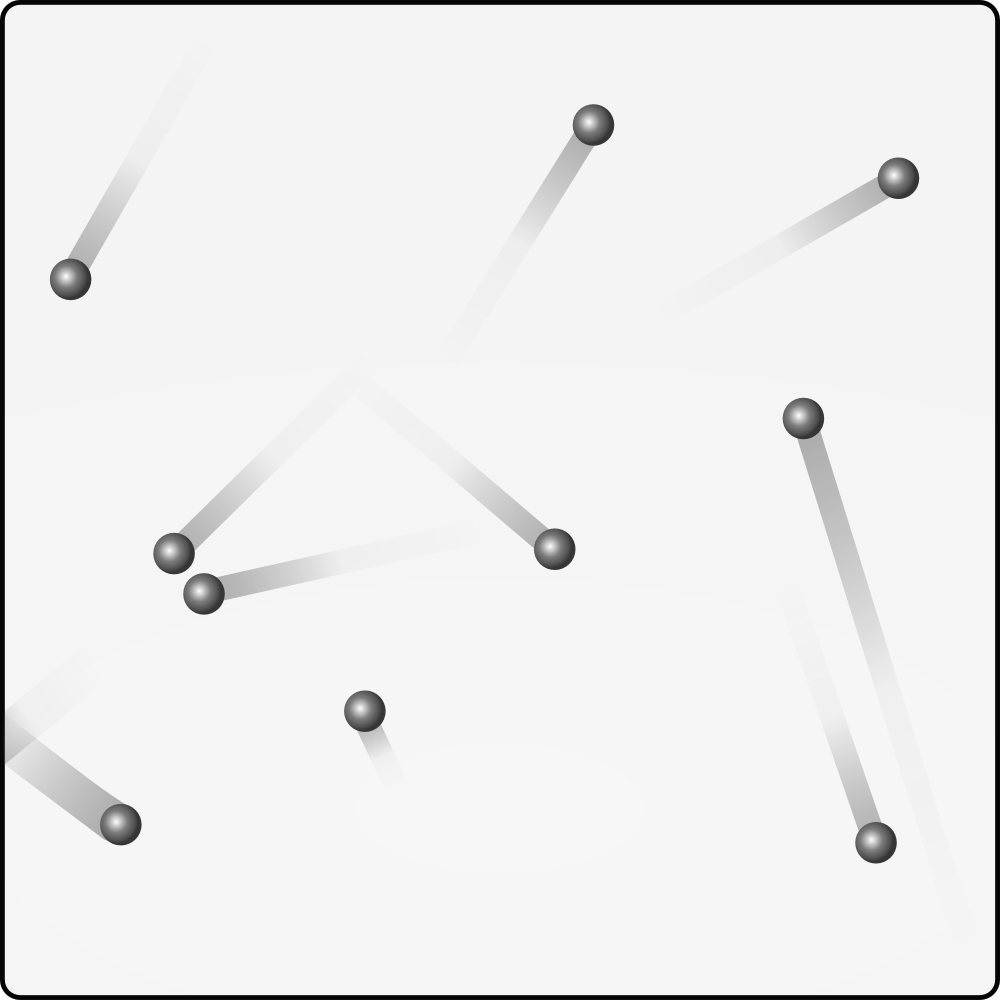
\includegraphics[width=8cm]{images/gaz_boules.png}
			\end{center}
			\supercaption{Un gaz parfait peut être visualisé comme un ensemble de boules en mouvement désordonné. Elles se percutent sans frottement et sans attraction mutuelle. La vitesse de chaque boule change à chaque heurt.}%
			{Dérivé d’\wcfile{Kinetic_theory_of_gases.svg}{un schéma} \ccbysa par \wcu{Sharayanan}}
			\label{fig_gaz_boules}
		\end{figure}
		
		Dans ce chaos, la température est une mesure de l’énergie cinétique des molécules. On la quantifie en mesurant la force résultant de l’impact des molécules sur une paroi du récipient --\ c’est-à-dire avec la pression. Avec ce modèle, nous pouvons proposer une échelle de température telle que $T \propto p$.
		
		Plus le nombre de molécules impactant la surface est faible, plus il faut qu’elles l’impactent fortement pour générer une pression donnée. Ainsi, lorsque la masse volumique $\rho$ diminue à une pression donnée, c’est que la température augmente. On peut donc également proposer $T \propto \frac{1}{\rho}$.
		
		Si ces deux propositions sont réunies en une seule équation, nous obtenons un modèle simple pour quantifier la température : $T \propto p v$.
		
		
	\subsection{Que ne représente pas un gaz parfait ?}
	\label{ch_pas_gaz_parfait}
	
		\thermoquotebegin{O}
			Quiconque veut étudier les propriétés de la matière dans un problème réel peut désirer partir en écrivant les équations fondamentales et puis essayer de les résoudre mathématiquement. Bien qu’il y ait des gens qui essayent d’emprunter une telle approche, ces personnes sont des ratés de ce domaine ; les véritables réussites sont le fait de ceux qui partent d’un point de vue \emph{physique}, de ceux qui ont une idée approximative de l’endroit où ils vont et qui commencent en faisant la bonne approximation, sachant ce qui est grand et ce qui est petit dans une situation donnée qui est compliquée.
		\thermoquoteend{Richard Feynman, 1963}{\textit{The Feynman Lectures on \mbox{Physics}} \mbox{\cite{feynman1963, feynman1963fr}}}
	
		Le comportement des molécules lorsqu’elles sont proches les unes des autres est en réalité très complexe, car les forces d’attraction y jouent un rôle déterminant. L’influence de ces forces est d’autant plus grande que les molécules sont lentes et structurellement complexes (l’interaction entre deux molécules d’hydrocarbone, par exemple, est plus difficile à modéliser que l’interaction entre deux molécules d’hélium).

		Les conséquences à l’échelle macroscopique de ces interactions, et les conditions dans lesquelles elles ne doivent plus être négligées, font l’objet du \courscinq.

		Nous retiendrons pour l’instant que le modèle du gaz parfait fonctionne mieux :

		\begin{itemize}
			\item Lorsque les molécules se percutent à grande vitesse, c’est-à-dire lorsque la température du gaz est élevée ;
			\item Lorsque l’espace moyen entre les molécules est grand, c’est-à-dire lorsque le volume spécifique du gaz est grand.
		\end{itemize}
		
		Ces conditions permettent de s’assurer que les forces d’attraction entre molécules gardent un rôle mineur dans le comportement global du gaz. Elles sont respectées pour l’air dans la grande majorité des applications en ingénierie. Nous utiliserons la valeur $R_\text{air} = \SI{287}{\joule\per\kilogram\per\kelvin}$ pour l’air pur dans nos machines.


	\subsection{Limites du modèle}

		Il ne faudra pas longtemps à l’étudiant/e pour trouver les limites de l’\cref{eq_pV=mRT}, qui indique qu’une masse non-nulle de gaz parfait occupe \textit{un volume nul} à température nulle. Strictement parlant, le gaz parfait ne peut pas exister --\ le modèle mathématique perd son sens à très basse température puisqu’il ne tient pas compte du volume des molécules elles-mêmes.

		Plusieurs autres équations d’état peuvent être utilisées pour correspondre aux gaz réels sur une plus grande plage de propriétés.

		Ainsi, l’\vocab{équation de Van der Waals}, proposée dès la fin du \textsc{xviii}\ieme siècle, propose :
		\begin{equation}
			\left(p + \frac{a}{v ^2}\right) (v - b) = R T
		\end{equation}
		\begin{equationterms}
			\item où $a$ et $b$ sont deux constantes.
		\end{equationterms}

		Cette équation a l’intérêt de tenir compte de deux facteurs ignorés dans l’équation d’état~\ref{eq_pv=RT} : la force d’attraction entre les molécules (le terme $a/v^2$, qui devient partie de l’expression de la pression) et le volume occupé par les molécules elles-mêmes (le terme $b$ qui se retranche au volume disponible).

		Malgré les difficultés inhérentes à la quantification des termes $a$ et $b$, ces modifications ont considérablement étendu la plage d’application des équations d’état. Elles ont valu à leur auteur, \wf{Johannes Diderik van der Waals}, le prix Nobel de physique en 1910.

		La recherche de modèles mathématiques pour décrire l’état des gaz réels est un thème important de recherche en mécanique des fluides. L’étudiant/e curieux/se pourra consulter les équations d’état \wed{Real_gas\#Beattie.E2.80.93Bridgman_model}{de Beattie-Bridgeman}, \wed{Benedict\%E2\%80\%93Webb\%E2\%80\%93Rubin_equation}{de Benedict-Webb-Rubin} ou encore de Strobridge pour se faire un aperçu de la complexité croissante de cette branche. Nous resterons quant à nous à l’\cref{eq_pv=RT}.



\section{Propriétés des gaz parfaits}

	\subsection{Deux capacités calorifiques importantes}

		Nous avons déjà abordé la notion de capacité calorifique (ou «~chaleur massique~»), au premier chapitre (\ref{eq_def_capacité_calorifique_massique}). Elle se définit comme la quantité de chaleur nécessaire pour augmenter d’un Kelvin\footnote{Ou d’un degré Celsius, ces différences de température étant égales.}
		la température d’un kilo du corps. On a ainsi :
		\begin{equation}
			c = \frac{\diff q}{\diff T}
		\end{equation}
		\begin{equationterms}
			\item où \tab $c$ 		\tab\tab est la capacité calorifique spécifique (\si{\joule\per\kelvin\per\kilogram}),
			\item 	\tab $\diff q$ \tab la quantité infinitésimale de chaleur spécifique fournie (\si{\joule\per\kilogram}),
			\item et \tab $\diff T$ \tab la variation infinitésimale de température provoquée (\si{\kelvin}).
		\end{equationterms}

		Comme la température d’un gaz varie aussi lorsqu’il reçoit ou fournit du travail, il existe une infinité de façons de faire varier sa température d’un degré, en combinant chaleur et travail (\cref{fig_expérience_diff_chaleurs_massiques}). Chacune nécessite une quantité de chaleur unique ; il y a donc \textit{une infinité de chaleurs massiques} correspondantes.

		\begin{figure}
			\begin{center}
				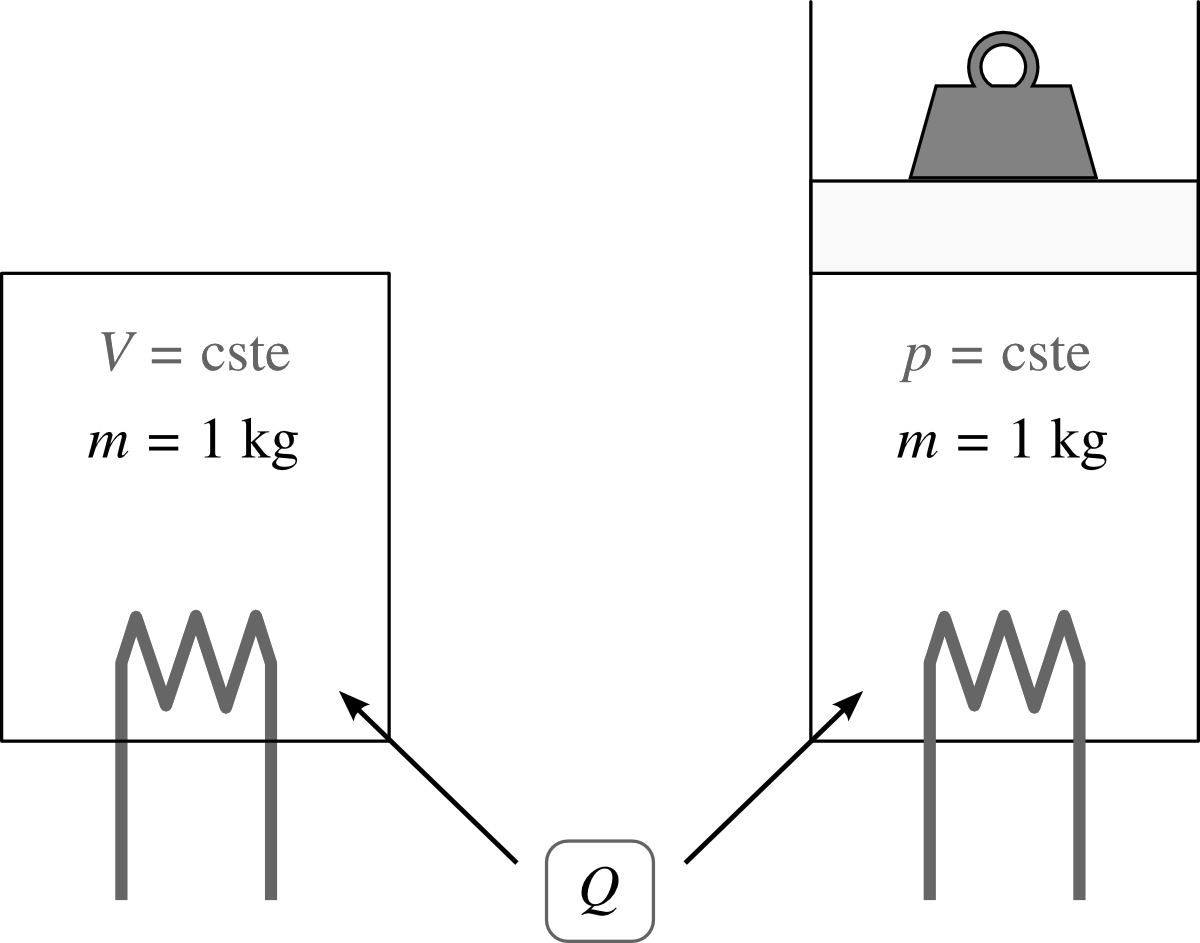
\includegraphics[width=10cm]{images/difference_capacites_calorifiques.png}
			\end{center}
			\supercaption{Deux quantités identiques de gaz reçoivent la même quantité de chaleur $Q$ . L’élévation de température sera plus faible à droite à cause du travail effectué sur le piston.}{schéma \cczero \oc}
			\label{fig_expérience_diff_chaleurs_massiques}
		\end{figure}

		Parmi celles-ci, deux valeurs particulières (\cref{fig_cp_et_cv}) nous servent de référence pour décrire le comportement d’un gaz parfait :

		\begin{figure}
			\begin{center}
				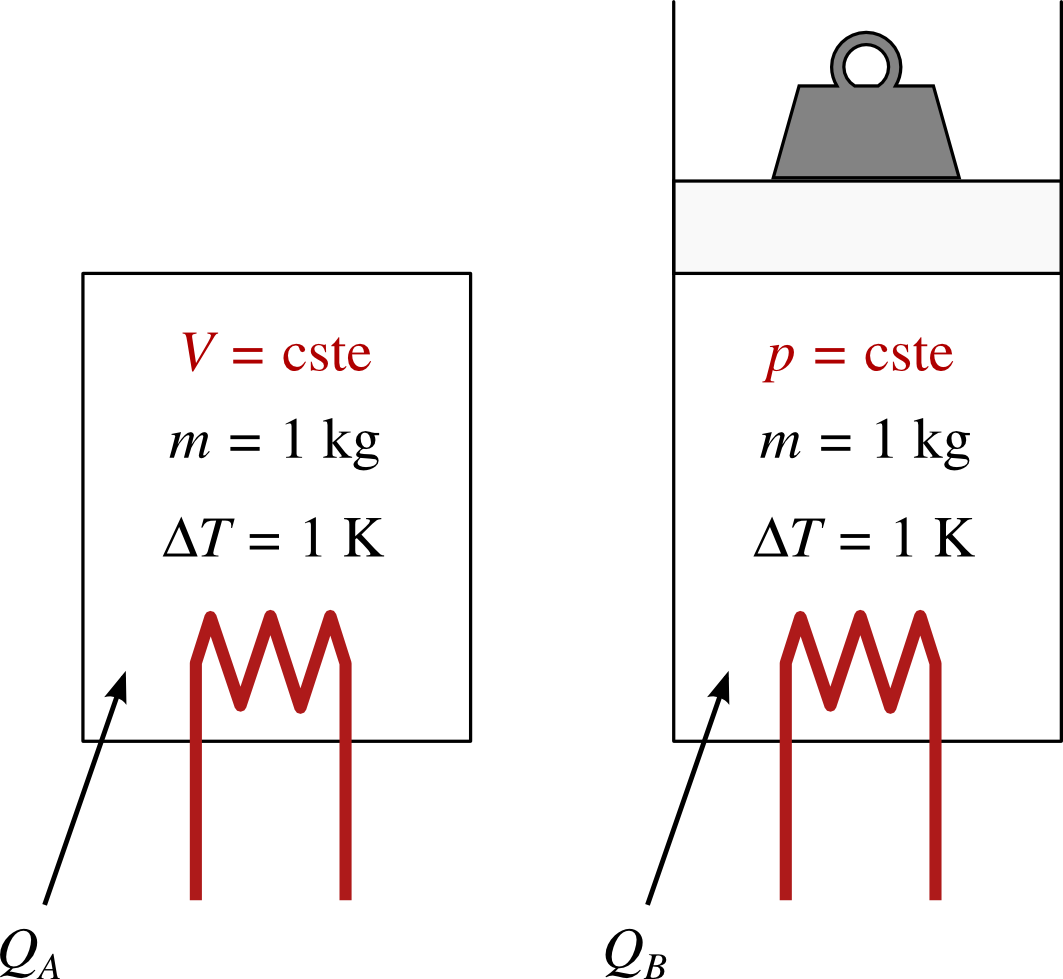
\includegraphics[width=9cm]{images/capacites_calorifiques.png}
			\end{center}
			\supercaption{Définitions des chaleurs massiques. À gauche, le volume est fixé et la capacité calorifique massique sera $c_v$. À droite, la pression est constante et la capacité sera $c_p$.}{schéma \cczero \oc}
			\label{fig_cp_et_cv}
		\end{figure}
		
		\begin{description}
			\item[la chaleur massique à volume constant :]$c_v$~, \dontbreakpage
			\item[la chaleur massique à pression constante :]$c_p$~.
		\end{description}

		Ces deux propriétés vont nous servir très bientôt pour quantifier l’énergie dans les gaz. $c_v$ et $c_p$ sont indépendantes de la température dans un gaz parfait. Dans les gaz réels, elles varient avec la température (\cref{fig_valeurs_de_cp_cv_gamma}), mais pour la plupart des applications en ingénierie il est raisonnable d’utiliser des valeurs moyennes. Pour l’air, nous retenons $c_{v\text{(air)}} = \SI{718}{\joule\per\kilogram\per\kelvin}$ et $c_{p\text{(air)}} = \SI{1005}{\joule\per\kilogram\per\kelvin}$.

		\begin{figure}
			\begin{center}
				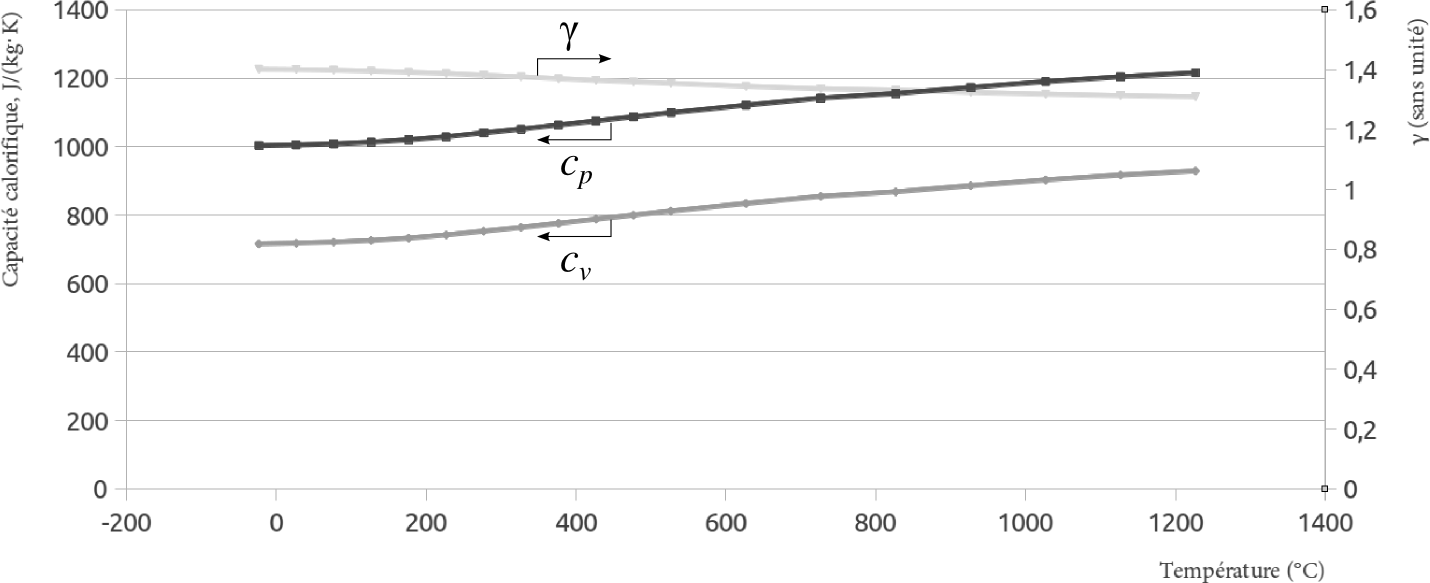
\includegraphics[width=15cm, inner]{images/valeurs_cp_cv_air.png}
			\end{center}
			\supercaption{Capacité calorifique de l’air en fonction de sa température. On note une variation sensible des valeurs dans la gamme de températures utilisée en ingénierie, que nous négligerons dans le cadre de notre étude de la thermodynamique.}%
				{Données issues du circulaire NBS 564 “Tables of Thermal Properties of Gases” (1955) jusqu’à~\SI{1000}{\kelvin}, calculées selon le modèle de B. G. Kyle in “Chemical and Process Thermodynamics” (1984) ensuite, et publiées par Israel Urieli (\href{http ://www.ohio.edu/mechanical/thermo/}{ohio.edu/mechanical/thermo/})}
		\label{fig_valeurs_de_cp_cv_gamma}
		\end{figure}




	\subsection{Différence des chaleurs massiques}

		Le grand nombre d’équations que nous abordons rend utile, mais pas indispensable, cette courte section. Pour l’ingénieur/e, il n’a d’autre intérêt que de permettre d’alléger l’écriture des relations de la section suivante.

		Observons les quantités d’énergie en jeu dans l’expérience décrite en \cref{fig_cp_et_cv}. Nous fournissons à chaque corps une quantité de chaleur différente pour obtenir la même variation de température. La différence entre les deux quantités de chaleur requises provient du fait que le gaz à pression constante (à droite) a fourni un travail pendant l’évolution.

		Quelle est la différence entre les chaleurs massiques de chacun des gaz ? Dans chacun des deux cas, nous avons $q_{1 \to 2} + w_{1 \to 2} = \Delta u$ (\ref{eq_premier_principe_sf_min}). Pour le corps A à gauche, comme aucun travail n’est effectué et que l’évolution est à volume constant, nous pouvons écrire :
			\begin{equation}
				\left\{
					\begin{array}{rl}
						q_\A 		& = c_v \ \Delta T \\
						\Delta u 			& = q_\A
					\end{array} \right.
			\label{eq_sectionmathschiante_0}
			\end{equation}

		Pour le corps B à droite, comme la pression $p_\text{cste}$ est constante, nous pouvons écrire :
			\begin{equation}
				\left\{
					\begin{array}{rl}
						q_\B 		& = c_p \ \Delta T \\
						\Delta u 	& = q_\B + (-p_\text{cste} \ \Delta v)
					\end{array} \right.
			\label{eq_sectionmathschiante_1}
			\end{equation}


		En combinant les deux systèmes~\ref{eq_sectionmathschiante_0} et~\ref{eq_sectionmathschiante_1}%
			\footnote{En étant véritablement rigoureux, pour affirmer que $\Delta u_A$ et $\Delta u_B$ sont égaux, il nous faudrait attendre l’\cref{eq_principe_de_joule} qui arrive à la section suivante.}%
		, nous obtenons
		\begin{equation}
			c_v \ \Delta T = c_p \ \Delta T - p_\text{cste} \ \Delta v
		\end{equation}

		qui stipule simplement que la différence entre les deux chaleurs fournies est retrouvée dans le travail fourni par le gaz de droite.

		Une brève manipulation amène :
		\begin{IEEEeqnarray}{rCl}
			(c_p - c_v) \Delta T 	& = & p_\text{cste} \ \Delta v	\nonumber \\
			(c_p - c_v) 				& = & \frac{pv_2 - pv_1}{\Delta T} = \frac{R T_2 - R T_1}{\Delta T} = \frac{R \ \Delta T}{\Delta T}	\nonumber \\
			c_p - c_v 					& = & R
		\label{eq_sectionmathschiante_2}
		\end{IEEEeqnarray}

		Cette expression a pour seul intérêt de nous permettre de simplifier l’\cref{eq_h_fonction_de_T} que nous allons écrire plus bas.


	\subsection{Quotient des chaleurs massiques}

		Le ratio des chaleurs massiques à pression et à volume constants est nommé $\gamma $. Ainsi :
		\begin{equation}
			\gamma \equiv \frac{c_p}{c_v}
			\label{def_gamma}
		\end{equation}

		En retournant à la \cref{fig_cp_et_cv} il apparaît rapidement que $c_p$ doit être supérieur à $c_v$ ; ainsi $\gamma$ est toujours supérieur à~\num{1}. Nous retenons $\gamma_\text{air} = \num{1,4}$.
		
		

\section{Énergie et température}

	\subsection{Contexte historique}
	
		\onlyframabook{\thermoquotebegin{O}%handmade citation remontée d’un paragraphe dans le framabook, sinon la mise en page est cassée
			M’étant assuré de ce fait important, que plus un espace est vide, et plus il s’en dégage de la chaleur lorsque l’air extérieur y pénètre, j’ai cherché à déterminer, par des expériences exactes, quelle relation il y avoit entre le calorique absorbé dans l’un des récipiens et celui dégagé dans l’autre, et comment ces variations de température dépendoient de celles de la variation de la densité de l’air.
		\thermoquoteend{Louis Joseph Gay-Lussac, 1807~\cite{gaylussac1807}}{\vspace{1em}}} %handmade vspace
	
		Au tout début du \textsc{xix}\ieme siècle ont lieu les premiers travaux de recherche visant à explorer la notion de température. La communauté scientifique s’intéresse alors beaucoup aux gaz -- on s’aperçoit qu’il y a \emph{deux} manières de faire augmenter leur température : en les chauffant, mais aussi en les comprimant.
		
		\onlyamphibook{\thermoquotebegin{O}%handmade la citation est ici au bon endroit, dans les Amphibooks seulement.
			M’étant assuré de ce fait important, que plus un espace est vide, et plus il s’en dégage de la chaleur lorsque l’air extérieur y pénètre, j’ai cherché à déterminer, par des expériences exactes, quelle relation il y avoit entre le calorique absorbé dans l’un des récipiens et celui dégagé dans l’autre, et comment ces variations de température dépendoient de celles de la variation de la densité de l’air.
		\thermoquoteend{Louis Joseph Gay-Lussac, 1807~\cite{gaylussac1807}}{\vspace{1em}}} %handmade vspace
		
		Le français \wf{Louis Joseph Gay-Lussac} cherche à comprendre pourquoi la température d’un gaz chute lorsqu’il se détend (il cherche en fait, selon les concepts d’alors, à identifier la source du \textit{calorique} et les raisons pour lesquelles il s’écoule). Il s’efforce ainsi de produire des détentes de gaz aussi simples que possible, et d’y mesurer la température. Une trentaine d’années plus tard, l’anglais \wf{James Prescott Joule} reprend et approfondit ces expériences\footnote{Les travaux méticuleux de Joule mèneront à la première expression formelle du premier principe de la thermodynamique, et à la fin de la théorie du \textit{calorique} selon laquelle la chaleur était un fluide très peu dense et invisible. Ils vaudront à son nom de famille l’utilisation que l’on sait aujourd’hui.} ; mais cette fois, en quantifiant la chaleur en tant qu’\textit{équivalence de travail}. Ces expériences avec ballons de gaz et thermomètres sont tout sauf spectaculaires -- mais elles vont jouer un rôle pivot en thermodynamique, parce qu’elles permettent de distinguer pour la première fois chaleur, travail, énergie et température.

	\subsection{La loi de Joule}
	\label{ch_principe_de_joule}

		\thermoquotebegin{O}
			J’ai pris deux ballons à deux tubulures, chacun de douze litres de capacité. A l’une des tubulures de chaque ballon étoit adapté un robinet, et à l’autre un thermomètre à alcool très-sensible, dont les degrés centigrades pouvoient être facilement divisés en centièmes. […] Le vide étant fait dans les deux ballons, et m’étant assuré qu’ils le retenoient exactement, je remplissois l’un d’eux avec le gaz sur lequel je voulois opérer. Environ douze heures après, j’établissois entre eux une communication au moyen d’un tuyau de plomb, et en ouvrant les robinets, le gaz se précipitoit alors dans le ballon vide jusqu’à ce que l’équilibre de pression fût rétablit de part et d’autre. Pendant ce tems, le thermomètre éprouvoit des variations que je notois avec soin.
		\thermoquoteend{Louis Joseph Gay-Lussac, 1807~\cite{gaylussac1807}}{\vspace{-1em}} %handmade vspace
		Dans leur expérience la plus remarquable, Joule et Gay-Lussac cherchent à faire varier la pression et le volume d’un gaz \textit{sans lui transférer de chaleur ou de travail}. Pour cela, ils laissent un gaz comprimé se détendre dans un second récipient vide (\cref{fig_detente_joule}). Le travail effectué est nul, car aucune surface n’a été déplacée – l’évolution est entièrement irréversible. La température est mesurée et… il ne se passe rien ! Joule et Gay-Lussac ne mesurent ni transferts de chaleur, ni variation de température.

		\begin{figure}
			\onlyframabook{\vspace{1.5em}}%handmade pour faire tenir la citation sur le côté
			\begin{center}
				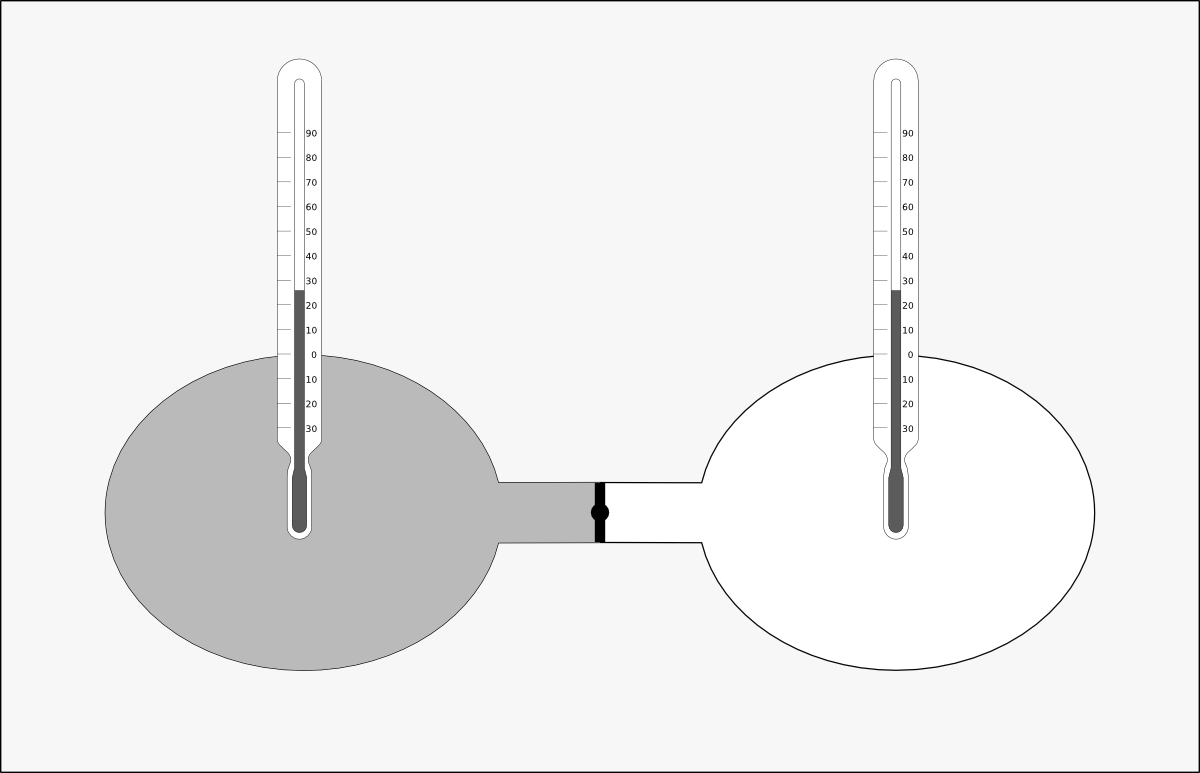
\includegraphics[width=9cm]{images/detente_joule_gay-lussac.png}
			\end{center}
			\supercaption{La \wfd{D\%C3\%A9tente de Joule-Gay-Lussac}{détente de Joule et Gay-Lussac}.\\			
		Un gaz est initialement prisonnier d’un réservoir à gauche ; on le laisse se détendre en ouvrant la vanne (au centre) qui le sépare d’un réservoir entièrement vide à droite.\\		
		Joule et Gay-Lussac s’intéressent aux variations de température mesurées dans chaque réservoir. Plus les propriétés du gaz rapprochent son comportement du modèle des gaz parfaits (\S\ref{ch_pas_gaz_parfait}), plus les variations de température qu’ils mesurent sont faibles, jusqu’à devenir indétectables pour certains gaz simples à haute température.}{schéma \cczero \oc}
			\label{fig_detente_joule}
		\end{figure}

		Joule effectue une multitude d’expériences différentes au cours desquelles il observe que quel que soit le travail fourni, la relation entre énergie interne (qui ne varie qu’avec travail et chaleur) et température reste sensiblement la même --\ et il suggère que pour un gaz parfait, elle reste toujours identique.

		Ce postulat est connu sous le nom de \vocab{loi de Joule} et est posé comme vrai pour tout gaz parfait. On peut le résumer ainsi :

		\begin{trucimportant}
			La température d’un gaz parfait ne varie qu’avec son énergie interne.
		\end{trucimportant}


		\thermoquotebegin{O}
La différence entre les moyennes des expansions et des expériences-témoin étant exactement telle que ce que à quoi nous avons attribué l’effet croissant de la température ambiante dans le dernier cas, nous arrivons à la conclusion qu’\emph{il n’y a pas de changement de température lorsque l’on laisse l’air se détendre d’une façon telle qu’il ne développe pas de puissance mécanique}.
		\thermoquoteend{James Joule, 1845~\cite{joule1845}}{}
		Mathématiquement, nous pouvons l’écrire ainsi :
		\begin{equation}
			u = f(T)
		\end{equation}

		La fonction $f$ peut être évaluée avec une expérience dans laquelle la variation de~$u$ est quantifiée. Par exemple, lors d’une évolution à volume constant $q = \Delta u$ et $q = c_v \ \Delta T$. On peut ainsi affirmer que la fonction $f$ est une simple relation de proportionnalité. L’énergie interne pouvant être arbitrairement posée comme nulle à température nulle ($u = \SI{0}{\joule\per\kilogram}$ lorsque $T = \SI{0}{\kelvin}$), on obtient :
		\begin{equation}
			u = c_v \ T
			\label{eq_principe_de_joule}
		\end{equation}
		\begin{equationterms}
			\item pour tout gaz parfait,
			\item quelle que soit l’évolution (réversible ou non),
			\item où \tab $u$ 	\tab est l’énergie interne spécifique (\si{\joule\per\kilogram}) ;
			\item 	\tab $T$ 	\tab est la température (\si{\kelvin}) ;
			\item et \tab $c_v$ 	\tab est la capacité calorifique massique à volume constant (\si{\joule\per\kilogram\per\kelvin}).
		\end{equationterms}

		Pour une masse $m$ de gaz parfait, on a bien sûr :
		\begin{equation}
			U = m \ c_v \ T
			\label{eq_principe_de_joule_m}
		\end{equation}

		Tant que notre fluide se comporte comme un gaz parfait, cette relation~\ref{eq_principe_de_joule} reste vraie. Elle fonctionne pendant toute évolution, réversible ou non, et quelles que soient les contraintes de volume, de pression ou de température.

		Par contre, il faut bien noter que cette \cref{eq_principe_de_joule}, qui découle de la loi de Joule, n’est pas du tout valable dans le cas des liquides et vapeurs. On peut, par exemple, ajouter de l’énergie à une masse d’eau bouillante, sans que sa température n’augmente. Nous étudierons les liquides et vapeurs dans le \courscinqshort.
		
		\begin{anexample}
			La chaleur massique à volume constant de l’air est mesurée à $c_{v\text{(air)}} = \SI{718}{\joule\per\kilogram\per\kelvin}$.\\
			On prend une masse de~\SI{0,5}{\kilogram} d’air à~\SI{20}{\degreeCelsius} et on lui transfère \SI{+15}{\kilo\joule} sous forme de chaleur et~\SI{-10}{\kilo\joule} sous forme de travail. Quelle est sa température finale ?
				\begin{answer}
					Nous savons que l’énergie a varié avec les transferts : $\Delta U = W_\fromatob + Q_\fromatob = m \ c_v \ \Delta T$. Ainsi, la température a varié en proportion : $T_\B = T_\A + \frac{\Delta U}{m \ c_v} = T_\A + \frac{W_\fromatob + Q_\fromatob}{m \ c_v} = \num{20} + \frac{\num{-10e3} + (\num{+15e3})}{\num{0,5} \times \num{718}} = \SI{33,92}{\degreeCelsius}$
				\end{answer}
					\begin{remark}Sacré James ! Il nous suffit de quantifier les variations d’énergie pour connaître la température, et vice-versa.\end{remark}
					\begin{remark}Ici les températures ne sont qu’additionnées et une conversion en \si{kelvins} n’aurait pas modifié le résultat. En cas de doute, il vaut mieux ne pas prendre ce raccourci. \end{remark}
		\end{anexample}



	\subsection{Enthalpie d’un gaz parfait}

		Parce que nous venons de lier l’énergie interne $u$ à la température et que le produit $p v$ dépend lui aussi de la température, nous pouvons désormais facilement exprimer l’enthalpie $h$ d’un gaz parfait en fonction de la température uniquement.

		En effet, nous avons $h \equiv u + p v$ (\ref{def_enthalpie}) ; avec une rapide insertion des équations~\ref{eq_pv=RT} et~\ref{eq_principe_de_joule} nous pouvons écrire, pour tout gaz parfait :
			\begin{equation}
				h = u + p v = c_v T + R T = (c_v + R) \ T
				\label{eq_h_fonction_de_T}
			\end{equation}

		Avec l’\cref{eq_sectionmathschiante_2} que nous avons développée plus haut, nous pouvons simplifier cette expression pour obtenir :
			\begin{equation}
				h = c_p \ T
				\label{eq_h=cpT}
			\end{equation}
			\begin{equationterms}
				\item Pour tout gaz parfait,
				\item quelle que soit l’évolution (réversible ou non),
				\item où \tab $h$ 	\tab est l’enthalpie spécifique (\si{\joule\per\kilogram}) ;
				\item 	\tab $T$ 	\tab est la température (\si{\kelvin}) ;
				\item et \tab $c_p$ 	\tab est la capacité calorifique massique à pression constante (\si{\joule\per\kilogram\per\kelvin}).
			\end{equationterms}
		
		
		\begin{anexample}
			La chaleur massique à pression constante de l’air est mesurée à $c_{p\text{(air)}} = \SI{1005}{\joule\per\kilogram\per\kelvin}$.\\
			Un débit de~\SI{2}{\kilogram\per\second} d’air passe dans un compresseur, où sa température augmente de~\SI{150}{\degreeCelsius}. Quelle est la puissance consommée par le compresseur ?
				\begin{answer}
					Nous savons que l’énergie est directement proportionnelle à la variation de température. Avec les équations \ref{eq_grande_sfee_deltas_h} et \ref{eq_h=cpT}, nous obtenons : $\dot W_\fromatob + \dot Q_\fromatob = \dot m \ \Delta h = \dot m \ c_p \ \Delta T = 2 \times \num{1005} \times (\num{+150}) = \SI{+301,5}{\kilo\watt}$.
				\end{answer}
					\begin{remark}Avec un gaz parfait, un simple thermomètre suffit pour quantifier l’énergie…\end{remark}
					\begin{remark}…mais pas pour différencier travail et chaleur. Ici nous ne pouvons pas séparer $\dot W_\fromatob$ de $\dot Q_\fromatob$. Nous ne pouvons pas non plus prédire l’état du gaz à la sortie, c’est à dire sa pression $p$ et son volume spécifique $v$ (seulement leur multiple). Pour cela, il faudrait une description précise de ce qui se passe entre l’entrée et la sortie.\end{remark}
		\end{anexample}


	\subsection{Interlude : Que retenir du gaz parfait jusqu’ici ?}

		Le gaz parfait est un modèle pour quantifier la température d’un gaz. Selon ce modèle, les trois principales formes d’énergie que nous avons utilisées jusqu’à présent —~l’énergie interne~$u$, l’enthalpie spécifique~$h$ et le terme~$p v$~— sont directement proportionnelles à la température~$T$ :
		\begin{IEEEeqnarray*}{rClC}
			u 	& = & c_v T 	& \qquad (\si{\joule\per\kilogram})	\\
			h 	& = & c_p T	& \qquad (\si{\joule\per\kilogram}) 	\\
			p v 	& = & R T 	& \qquad (\si{\joule\per\kilogram})
		\end{IEEEeqnarray*}

		Si l’on mesure la température absolue d’un gaz, alors on peut quantifier immédiatement ces trois formes d’énergie.




\section{Transformations élémentaires réversibles}
\label{ch_gp_evolutions_elementaires}

	Nous nous proposons ici de calculer les propriétés d’un gaz parfait, ainsi que les transferts d’énergie en jeu, lorsqu’on le comprime ou détend selon des contraintes entièrement arbitraires de volume, pression ou température.


	\subsection{À quoi sert cette section de chapitre ?}
	\label{ch_gp_evolutions_elementaires_aquoisert}

		Les évolutions de gaz que nous étudions ici sont très hypothétiques et pas nécessairement passionnantes, mais elles méritent l’attention de l’étudiant/e pour deux raisons :

		\begin{enumerate}
			\item Le comportement d’un gaz, même avec le modèle du gaz parfait, est intrinsèquement complexe. Ces évolutions élémentaires font figure de gymnastique et permettent d’apprendre à le décrire étape par étape ;
			\item Ces évolutions élémentaires sont des outils conceptuels que nous assemblerons plus tard, d’abord pour quantifier les limites théoriques des machines (au \coursseptshort), puis pour décrire le comportement des gaz à l’intérieur des machines réelles (au \coursdixshort).
		\end{enumerate}


	\subsection{Évolutions à pression constante}
	\label{ch_gp_isobares}

		Il est possible de chauffer ou refroidir un gaz en maintenant sa pression constante (\cref{fig_gp_pression_constante}). Une évolution à pression constante est dite \vocab{isobare}. Pour générer une telle transformation, nous pouvons :
		
		\begin{itemize}
			\item avec un système fermé, chauffer ou refroidir le gaz en maintenant une force constante sur les parois ;
			\item avec un système ouvert, chauffer ou refroidir le gaz en le laissant simplement s’écouler dans un conduit, sans pièce mobile. C’est le cas par exemple dans la chambre de combustion d’un turboréacteur.
		\end{itemize}

		\begin{figure}
			\begin{center}
				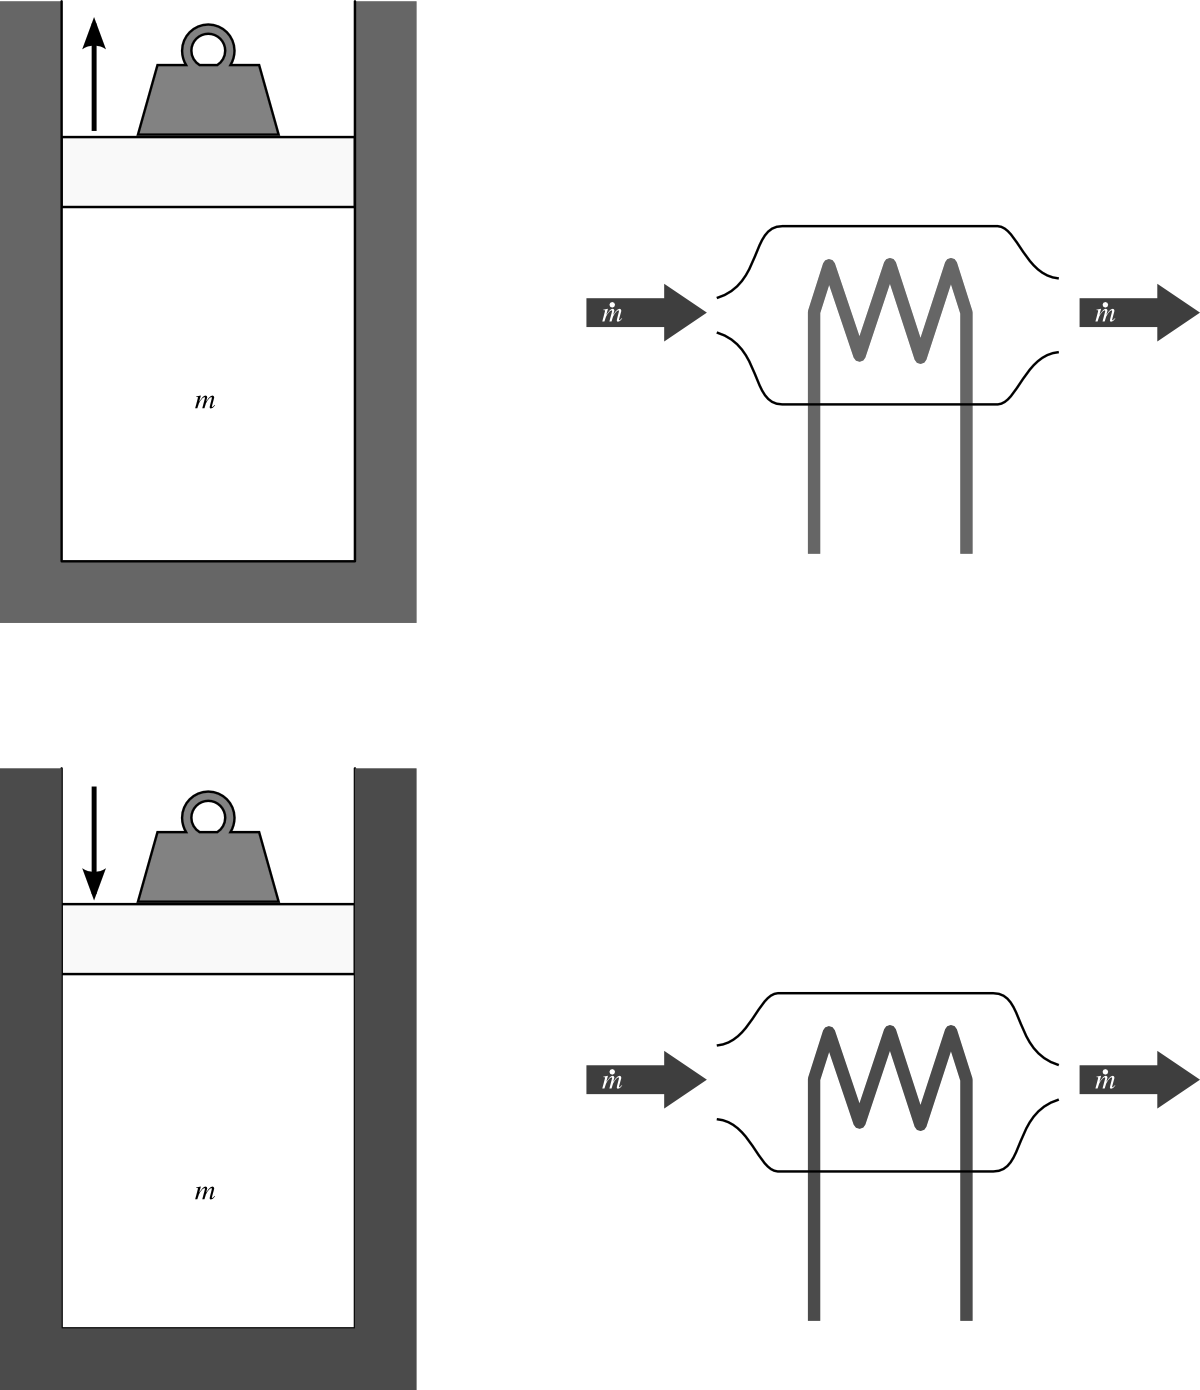
\includegraphics[width=8cm]{images/pression_constante.png}
			\end{center}
			\supercaption{Évolution à pression constante (isobare) d’un gaz parfait. En système fermé (à gauche), le piston exerce une force constante tout au long de l’évolution. En système ouvert (à droite), aucun travail n’est effectué.}{\cczero \oc}
			\label{fig_gp_pression_constante}
		\end{figure}
		
		\begin{figure}
			\begin{center}
				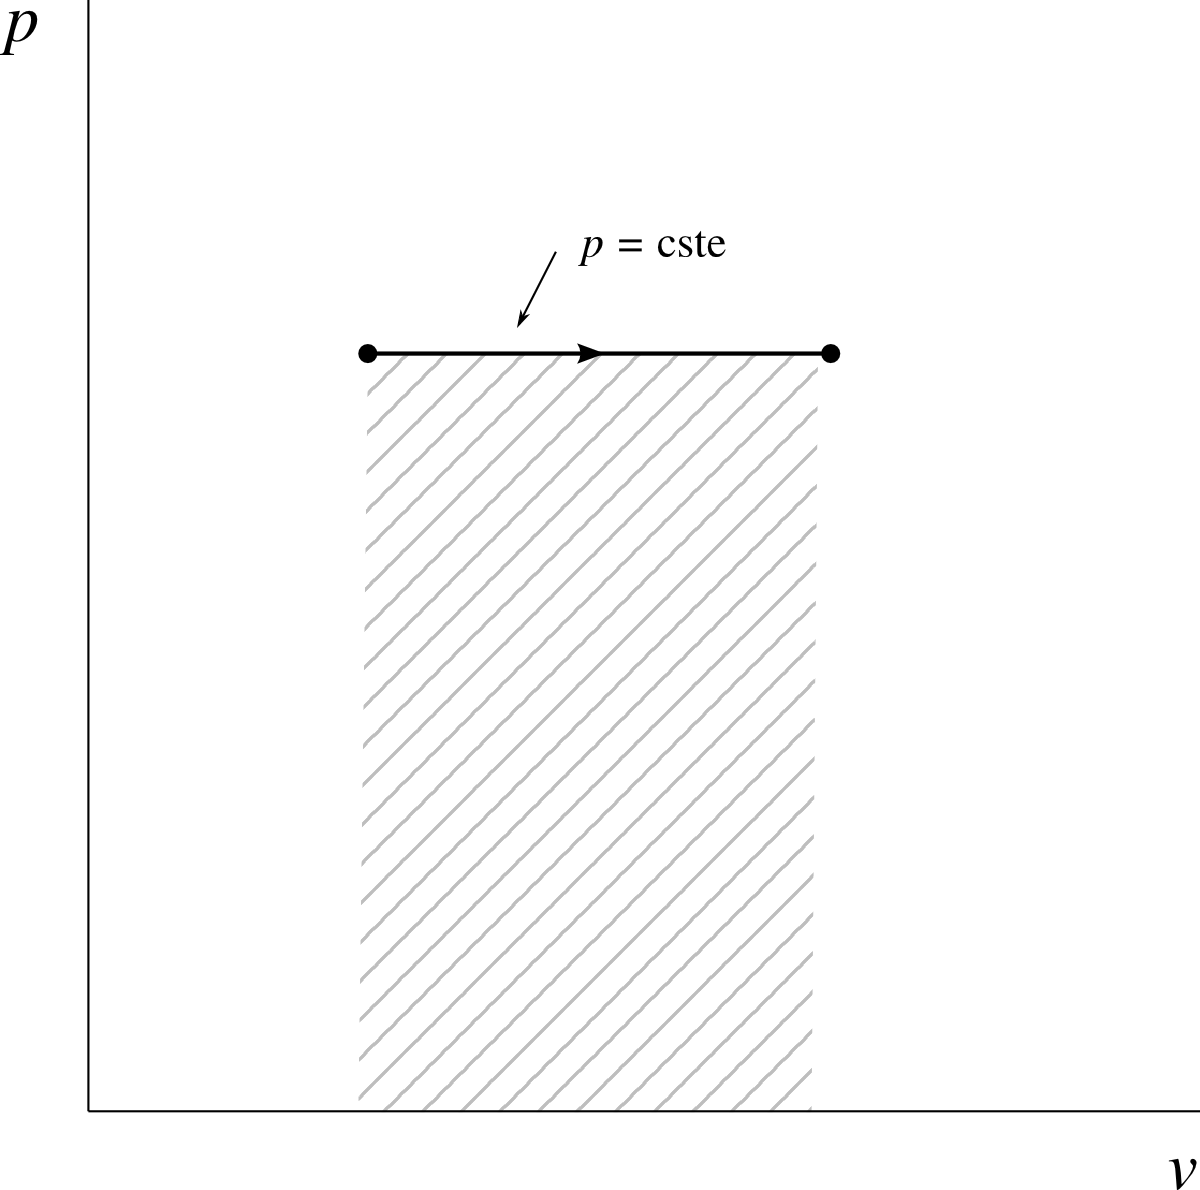
\includegraphics[width=\pvdiagramwidth]{images/pv_isobare.png}
			\end{center}
			\supercaption{Réchauffement à pression constante d’un gaz parfait, représenté sur un diagramme pression-volume.}{\cczero \oc}
			\label{fig_gp_pression_constante_pv}
		\end{figure}		

		Lorsque la pression est constante, les propriétés du gaz varient selon la relation
		\begin{equation}
			\frac{T}{v} = \text{constante}
		\end{equation}
		
		
		En système fermé, nous avons $q_{1\to2} + w_{1\to2} = \Delta u$ (\ref{eq_premier_principe_sf_min}) et, si l’évolution est réversible, la chaleur et le travail peuvent être facilement reliés à la température :
		\begin{IEEEeqnarray}{rCl}
			w_{1\to2} 	& = & - \int _1^2 p \diff v = -p_\text{cste} \int _1^2 \diff v = -p_\text{cste} \ \Delta v	\nonumber \\
			w_{1 \to 2} 	& = & - R \ \Delta T
		\end{IEEEeqnarray}
		\begin{equationterms}
			\item lors d’une évolution réversible à pression constante $p_\text{cste}$, en système fermé.
		\end{equationterms}

		On remarque que le travail est de signe opposé à la variation de température.
		
		La chaleur peut être quantifiée aisément :
		\begin{IEEEeqnarray}{rCl}
			q_{1\to2} 	& = & \Delta u - w_{1\to2} = \Delta u + p_\text{cste} \ \Delta v = \Delta h \nonumber \\
			q_{1 \to 2} 	& = & c_p \ \Delta T \label{eq_q_gp_sf_isobare}
		\end{IEEEeqnarray}
		\begin{equationterms}
			\item lors d’une évolution réversible à pression constante, en système fermé.
		\end{equationterms}

		
		Lorsque l’évolution se fait en système ouvert, nous avons $q_{1\to2} + w_{1\to2} = \Delta h$ (\ref{eq_petite_sfee_deltas_h}), et, si l’évolution est réversible, la chaleur et le travail se quantifient sans peine :		
		\begin{IEEEeqnarray}{rCl}
			w_{1\to2} 	& = & \int _1^2 v \diff p \nonumber \\
			w_{1\to2} 	& = & 0
		\end{IEEEeqnarray}
		\begin{equationterms}
			\item lors d’une évolution réversible à pression constante, en système ouvert.
		\end{equationterms}

		Le travail est bien sûr nul, puisqu’aucune pièce mobile n’est présente pour extraire de l’énergie mécanique du gaz.

		La chaleur est alors responsable de l’entièreté de la variation de température :
		\begin{IEEEeqnarray}{rCl}
			q_{1\to2} 	& = & \Delta h - w_{1\to2} = \Delta h \nonumber \\
			q_{1 \to 2} 	& = & c_p \ \Delta T \label{eq_q_gp_so_isobare}
		\end{IEEEeqnarray}
		\begin{equationterms}
			\item lors d’une évolution réversible à pression constante, en système ouvert.
		\end{equationterms}

		\begin{anexample}
			Pour l’air, on mesure $c_{p\text{(air)}} = \SI{1005}{\joule\per\kilogram\per\kelvin}$, $c_{v\text{(air)}} = \SI{718}{\joule\per\kilogram\per\kelvin}$, $R_\text{air} = \SI{287}{\joule\per\kilogram\per\kelvin}$.
			Combien faut-il d’énergie pour chauffer l’air dans un appartement de~\SI{30}{\metre\squared} depuis \SI{10}{\degreeCelsius} jusqu’à \SI{20}{\degreeCelsius} ?
				\begin{answer}
					Le réchauffement se fera vraisemblablement à pression constante (à moins que l’appartement ne soit fermé hermétiquement, la pression sera partout atmosphérique et l’air «~fuira~» sous les portes). Nous supposons une pression de~\SI{1}{\bar} et une hauteur de plafond de~\SI{2,5}{\metre}. Nous utilisons un système fermé englobant tout l’air réchauffé.
					
					Nous avons un volume de~\SI{75}{\metre\cubed}, ce qui mène la masse totale d’air à $m_\A = \frac{p_\A \ V_\A}{R \ T_\A} = \frac{\num{1e5} \times \num{75}}{\num{287} \times (\num{10} + \num{273,15})} = \SI{92,29}{\kilogram}$.\\
					La chaleur nécessaire pour chauffer cette quantité d’air à pression constante est quantifiable avec l’\cref{eq_q_gp_sf_isobare} : $Q_\fromatob = m \ c_p \ \Delta T = \num{93,29} \times \num{1005} \times (\num{20} - \num{10}) = \SI{+9,28e5}{\joule} = \SI{+928}{\kilo\joule}$.
				\end{answer}
					\begin{remark}Ce résultat représente le transfert final \emph{net} de chaleur vers l’air (incluant les pertes vers les murs et les fenêtres, ainsi que les transferts qui les compensent).\end{remark}
					\begin{remark}À l’inverse, un refroidissement provoquerait l’arrivée d’air extérieur, dont il faudrait tenir compte dans le calcul de la masse.\end{remark}
		\end{anexample}

	\subsection{Évolutions à volume constant}
	\label{ch_gp_isochores}

		Il est possible de chauffer ou refroidir un gaz en maintenant son volume constant (\cref{fig_gp_volume_constant}). Une évolution à volume constant est dite \vocab{isochore}.
			
		\begin{itemize}
			\item Avec un système fermé, nous pouvons chauffer ou refroidir un gaz dans un réservoir fixe et fermé. C’est le cas par exemple pendant la phase de combustion («~explosion~») dans un moteur à essence.
			\item Avec un système ouvert, la manipulation est plus complexe. Nous devons compresser le gaz pendant qu’on le réchauffe pour éviter que son volume n’augmente ; À l’inverse, pendant un refroidissement, il faut le détendre pour éviter que son volume ne baisse. Cette manipulation n’a pas d’application pratique courante.
		\end{itemize}	
		
		\begin{figure}
			\begin{center}
				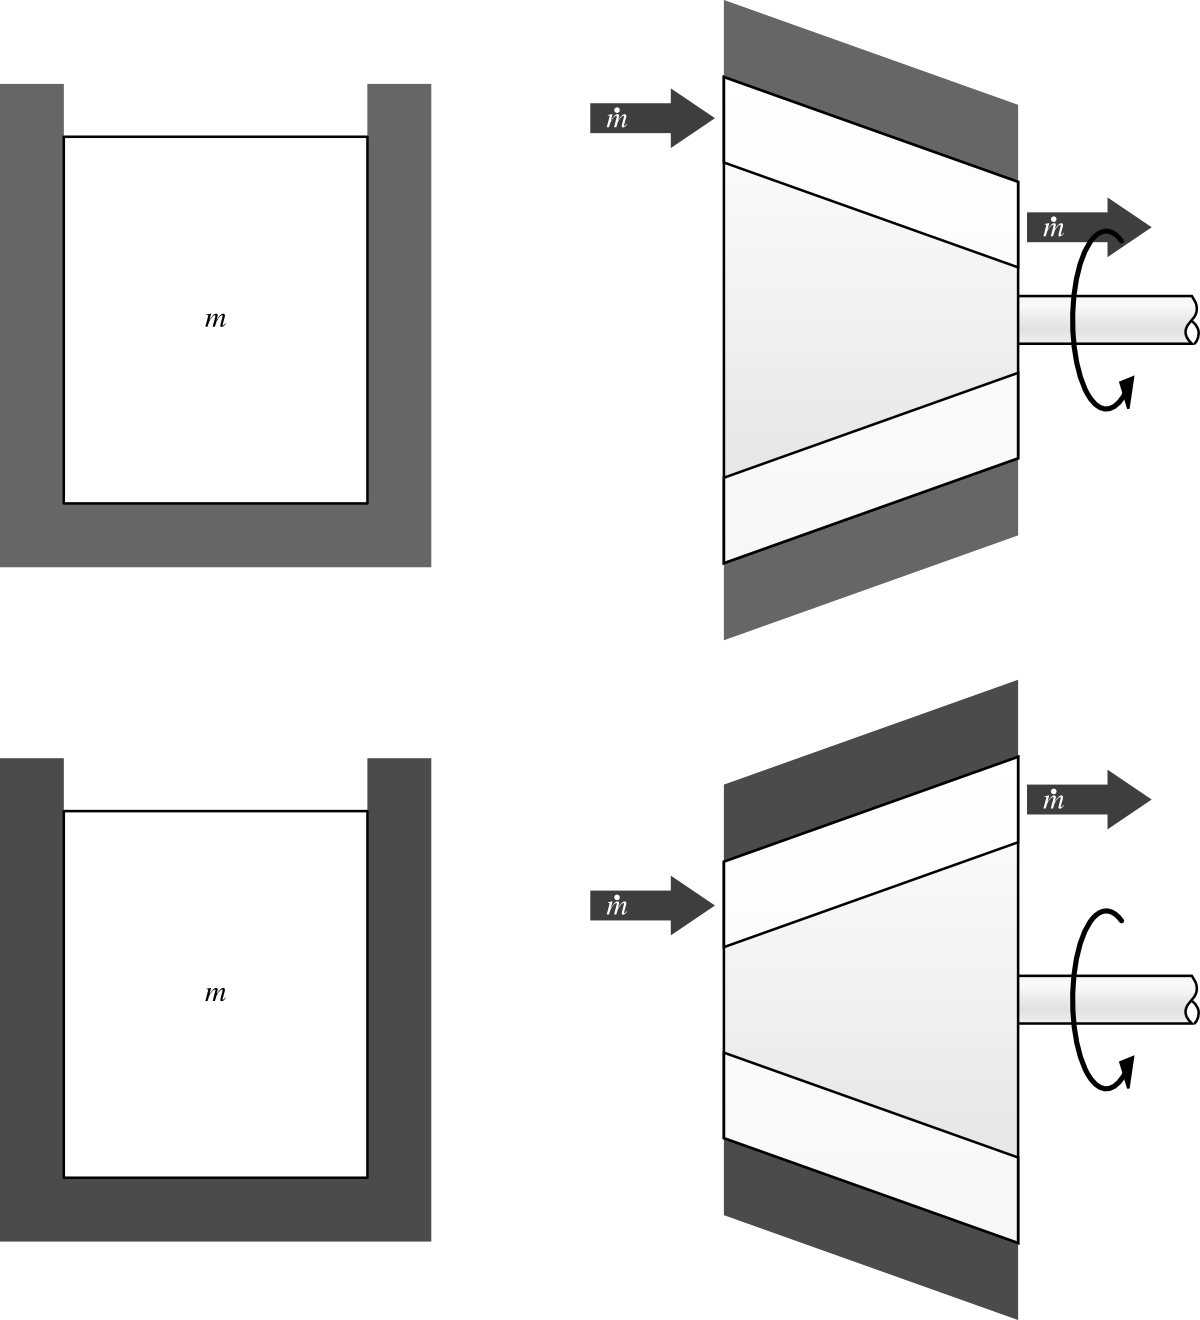
\includegraphics[width=8cm]{images/volume_constant.png}
			\end{center}
			\supercaption{Évolution à volume constant (isochore) d’un gaz parfait. En système fermé (à gauche), le volume est bloqué et aucun travail n’est effectué. En système ouvert (à droite), on doit comprimer le gaz pendant qu’on le chauffe et le détendre pendant qu’on le refroidit, pour pouvoir maintenir le volume spécifique constant.}{\cczero \oc}
			\label{fig_gp_volume_constant}
		\end{figure}
		
		\begin{figure}
			\begin{center}
				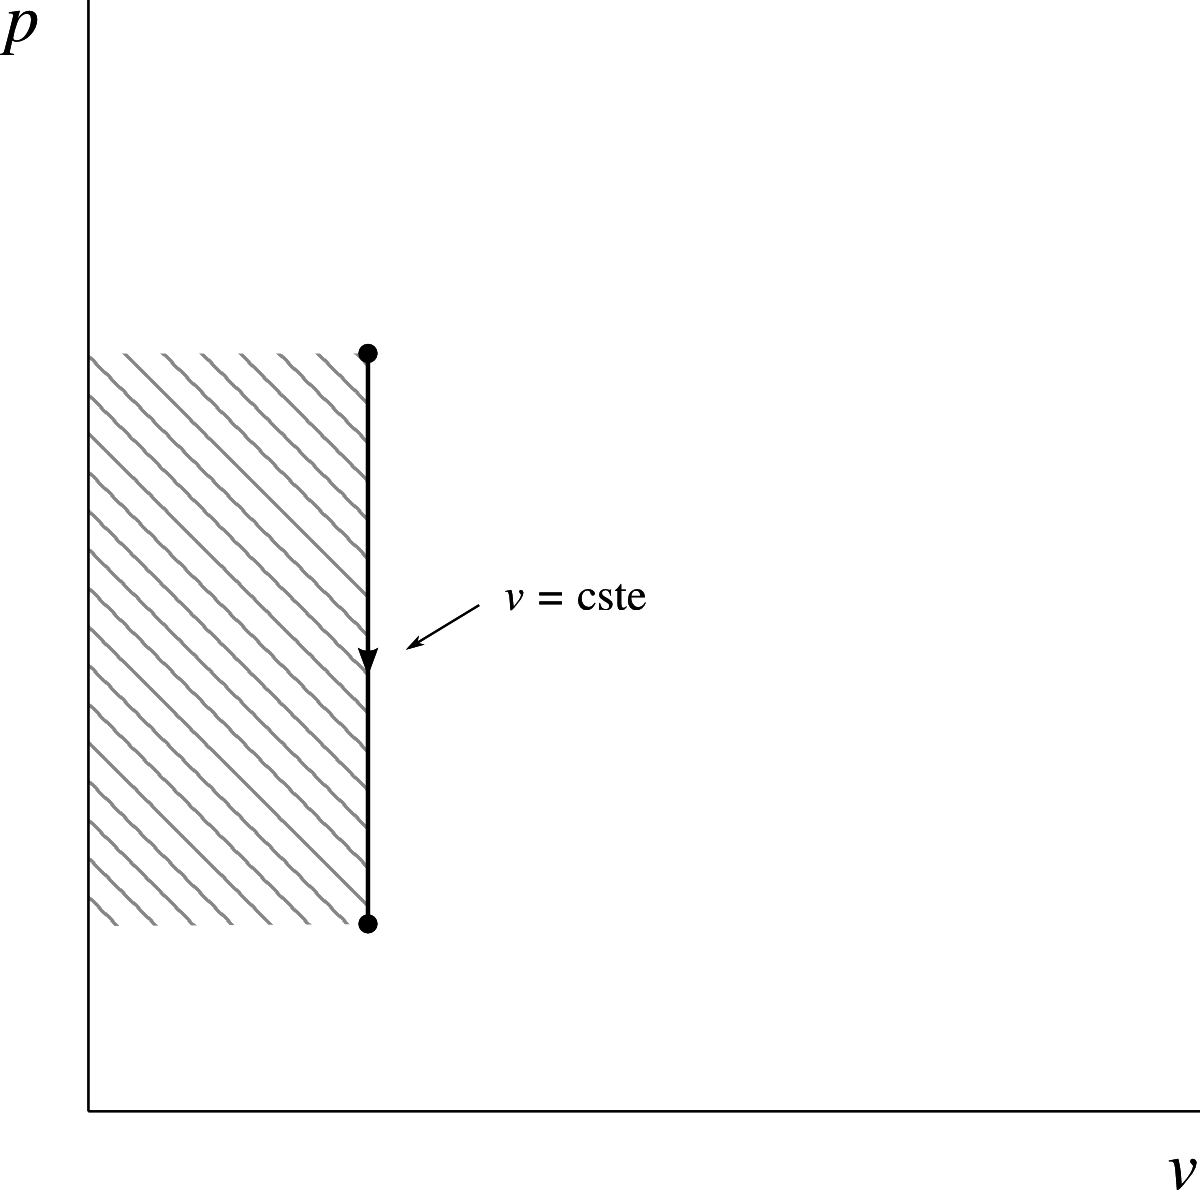
\includegraphics[width=\pvdiagramwidth]{images/pv_isochore.png}
			\end{center}
			\supercaption{Refroidissement à volume constant d’un gaz parfait, représenté sur un diagramme pression-volume.}{\cczero \oc}
			\label{fig_gp_volume_constant_pv}
		\end{figure}		

		Lorsque le volume spécifique d’un gaz parfait est constant, ses propriétés varient selon la relation
		\begin{equation}
			\frac{T}{p} = \text{constante} \label{eq_gp_isochore}
		\end{equation}
		
		En système fermé, nous avons $q_{1\to2} + w_{1\to2} = \Delta u$ et, si l’évolution est réversible, la chaleur et le travail peuvent être facilement reliés à la température.

		Le volume ne variant pas, le travail est bien sûr nul :
		\begin{IEEEeqnarray}{rCl}
			w_{1\to2} 	& = & - \int _1^2 p \diff v	\nonumber \\
			w_{1\to2} 	& = & 0 \label{eq_w_gp_sf_isochore}
		\end{IEEEeqnarray}
		\begin{equationterms}
			\item lors d’une évolution réversible à volume constant, en système fermé.
		\end{equationterms}

		La chaleur peut être quantifiée aisément :
		\begin{IEEEeqnarray}{rCl}
			q_{1\to2} 	& = & \Delta u - w_{1\to2} = \Delta u \nonumber \\
			q_{1\to2} 	& = & c_v \ \Delta T \label{eq_q_gp_sf_isochore}
		\end{IEEEeqnarray}
		\begin{equationterms}
			\item lors d’une évolution réversible à volume constant, en système fermé.
		\end{equationterms}

		
		Lorsque l’évolution se fait en système ouvert, nous avons $q_{1\to2} + w_{1\to2} = \Delta h$ et, si l’évolution est réversible, la chaleur et le travail peuvent être quantifiés, bien qu’avec un peu plus de difficulté :
		\begin{IEEEeqnarray}{rCl}
			w_{1\to2} 	& = & \int _1^2 v \diff p = v_\text{cste} \int_1^2 \diff p = v_\text{cste} \int_1^2 \frac{R}{v_\text{cste}} \diff T = R \int_1^2 \diff T \nonumber \\
			w_{1\to2} 	& = & R \ \Delta T
		\end{IEEEeqnarray}
		\begin{equationterms}
			\item lors d’une évolution réversible à volume constant, en système ouvert.
		\end{equationterms}

		On peut alors quantifier facilement la chaleur à fournir :
		\begin{IEEEeqnarray}{rCl}
			q_{1\to2} 	& = & \Delta h - w_{1\to2} = c_p \ \Delta T - R \ \Delta T \nonumber \\
			q_{1\to2} 	& = & c_v \ \Delta T
		\end{IEEEeqnarray}
		\begin{equationterms}
			\item lors d’une évolution réversible à volume constant, en système ouvert.
		\end{equationterms}

		\begin{anexample}
			Pour l’air, on mesure $c_{p\text{(air)}} = \SI{1005}{\joule\per\kilogram\per\kelvin}$, $c_{v\text{(air)}} = \SI{718}{\joule\per\kilogram\per\kelvin}$, $R_\text{air} = \SI{287}{\joule\per\kilogram\per\kelvin}$.\\
			Dans un cylindre de moteur à essence, de l’air se trouve à pression de~\SI{17}{\bar} avec une masse volumique de~\SI{9,4}{\kilogram\per\metre\cubed}. La combustion du carburant (si rapide que le volume n’a pas le temps de varier) se traduit par l’apport de~\SI{1450}{\kilo\joule\per\kilogram} de chaleur. Quelles valeurs atteignent la température et la pression ?
				\begin{answer}
					Au départ, la température est $T_\A = \frac{p_\A v_\A}{R} = \frac{p_\A}{\rho_A R} = \frac{\num{17e5}}{\num{9,4} \times \num{287}} = \SI{630,1}{\kelvin} = \SI{357}{\degreeCelsius}$.\\
					Nous utilisons un système fermé constitué par la masse d’air. Le volume ne variant pas, le travail est nul (\ref{eq_w_gp_sf_isochore}) et c’est la chaleur qui fait varier l’énergie interne (\ref{eq_q_gp_sf_isochore}) : $q_\fromatob = \Delta u - w_\fromatob = \Delta u = c_v \ \Delta T$ ; ainsi $T_\B = T_\A + \frac{q_\fromatob}{c_v} = \num{630,1} + \frac{\num{1450e3}}{\num{718}} = \SI{2649,6}{\kelvin} = \SI{2376,5}{\degreeCelsius}$.\\
					La pression finale s’obtient en comparant la condition finale et la condition initiale (\ref{eq_gp_isochore}) : $\frac{R T_\A}{p_\A} = v_\A = v_\B = \frac{R T_\B}{p_\B} $ ; ainsi $p_\B = \frac{T_\B}{T_\A} p_\A = \frac{\num{2649,6}}{\num{630,1}} \times \num{17e5} = \SI{7,148e6}{\pascal} = \SI{71,5}{\bar}$.
						\begin{remark}Attention à bien compter les températures en \si{kelvins} dans les fractions.\end{remark}
						\begin{remark}La température maximale, supérieure à~\SI{2300}{\degreeCelsius}, dépasse la température de fonte de la plupart des métaux. Dans un moteur à essence, cette température n’est atteinte que sporadiquement, à chaque combustion.\end{remark}
						\begin{remark}Les données de cet exemple imitent celles de l’exercice \ref{exo_cycle_moteur_essence}. Cette fois, nous savons prédire les conditions finales sans devoir faire de mesure.\end{remark}
				\end{answer}
		\end{anexample}

	\subsection{Évolutions à température constante}
	\label{ch_gp_isothermes}
	
		\thermoquotebegin{O}
			Il est facile d’imaginer une petite quantité de combustible gazeux ou liquide, ou bien de la poussière de charbon, que l’on insèrerait dans un volume d’air comprimé et très chaud, et qui brûlerait suite à un allumage séparé ou spontané. Le piston est chassé en même temps de sorte qu’aucune augmentation de température n’ait lieu, car la chaleur développée par chaque particule de combustible est instanément absorbée par le refroidissement dû à l’expansion. De cette façon l’ensemble de la chaleur est transformée en travail.
		\thermoquoteend{Rudolf Diesel, 1893}{\textit{Theorie und Konstruktion eines rationellen Wärmemotors zum Ersatz der Dampfmaschinen und der heute bekannten Verbrennungsmotoren}~\mbox{\cite{diesel1893,diesel1893en}}\vspace{5em}} %handmade vspace
		Il est possible de chauffer ou refroidir un gaz en maintenant sa température constante (\cref{fig_gp_température_constante}). Une évolution à température constante est dite \vocab{isotherme}.
		
		\begin{figure}
			\begin{center}
				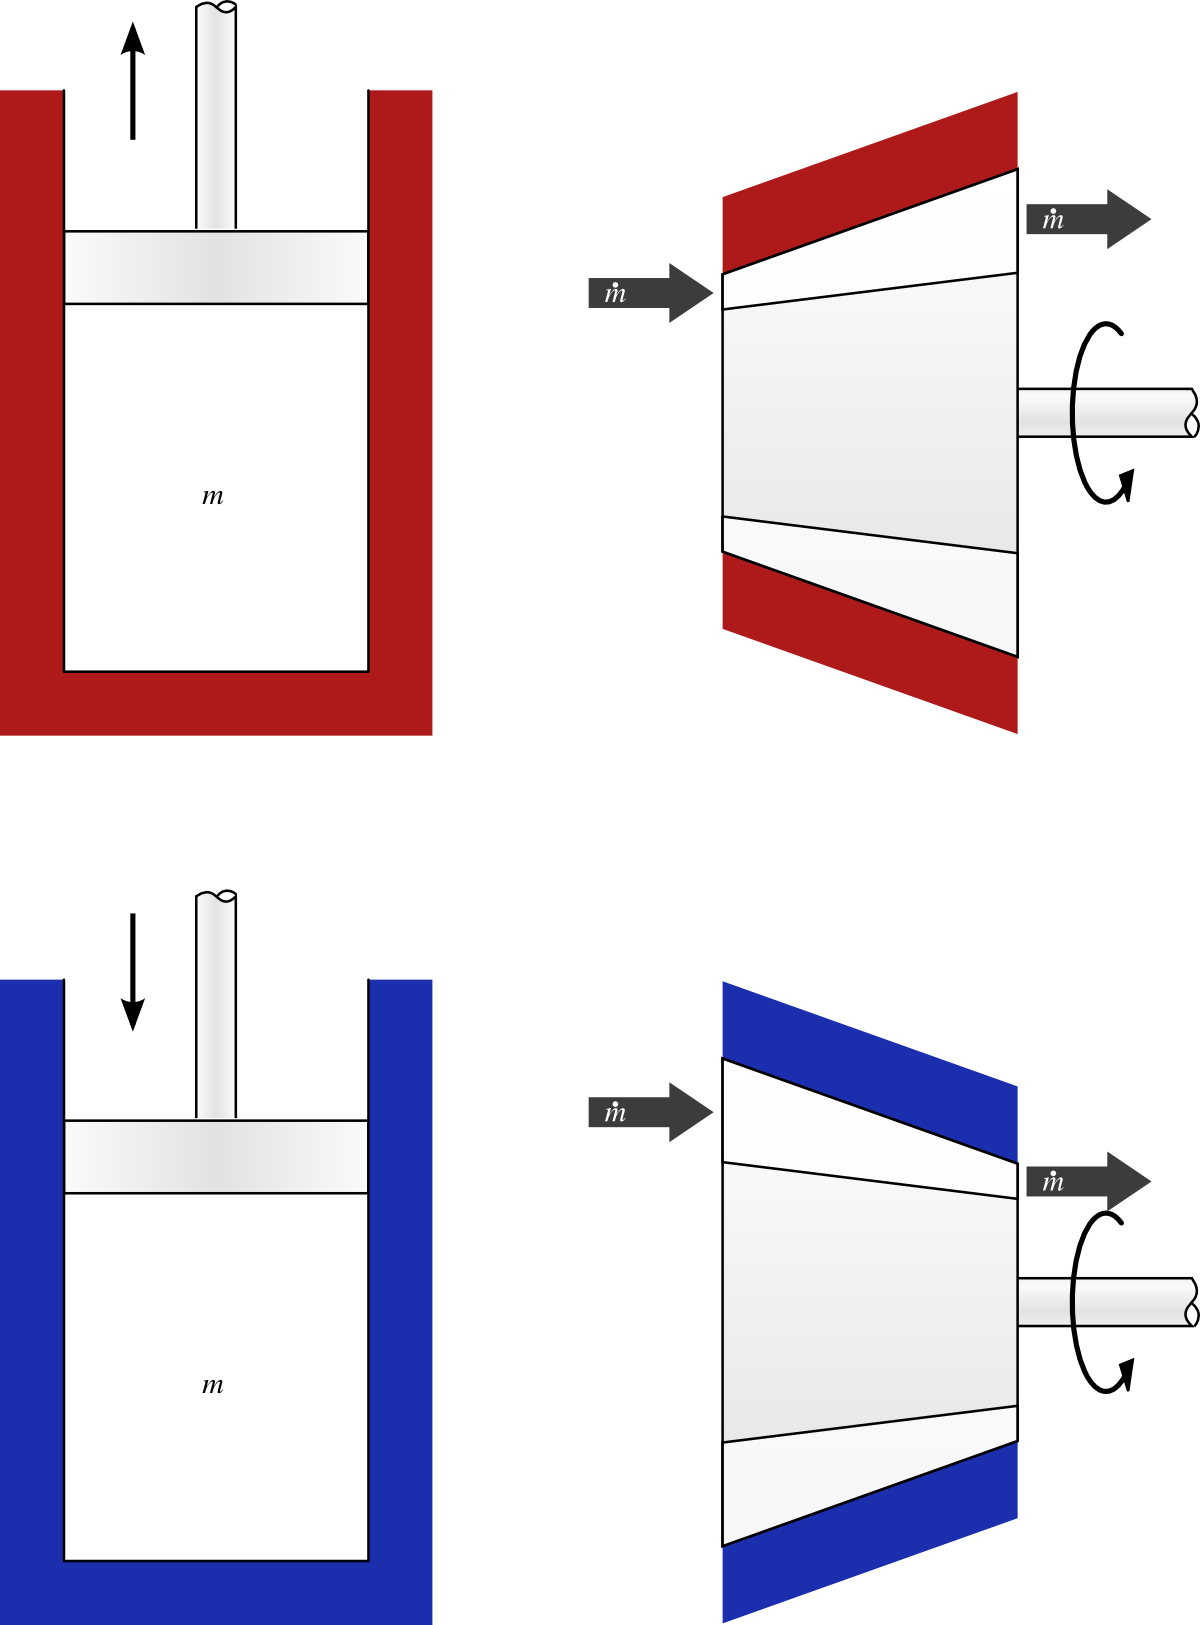
\includegraphics[width=8cm]{images/temperature_constante.png}
			\end{center}
			\supercaption{Évolution à température constante (isotherme) d’un gaz parfait. En système fermé (à gauche), on laisse travailler le gaz sur un piston pendant qu’on le chauffe, et à l’inverse, on lui fournit du travail lorsqu’on le refroidit. En système ouvert (à droite), les mêmes manipulations sont effectuées en flux continu.}{\cczero \oc}
			\label{fig_gp_température_constante}
		\end{figure}
		
		\begin{figure}
			\begin{center}
				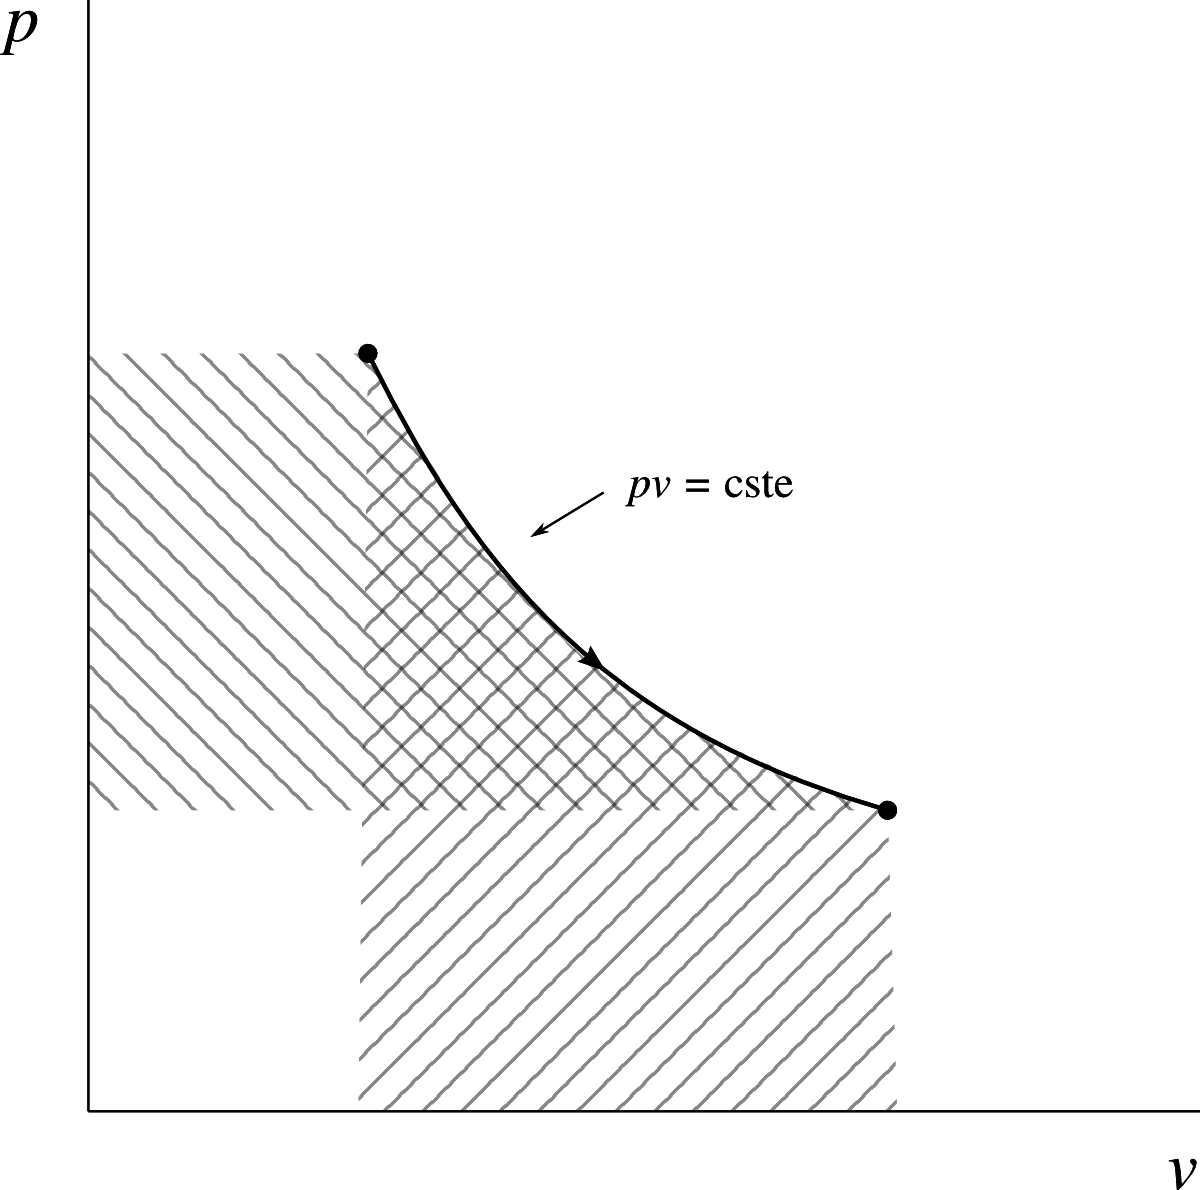
\includegraphics[width=\pvdiagramwidth]{images/pv_isotherme.png}
			\end{center}
			\supercaption{Détente (réchauffement) à température constante d’un gaz parfait, représenté sur un diagramme pression-volume.}{\cczero \oc}
			\label{fig_gp_température_constante_pv}
		\end{figure}		

		Pour un gaz parfait, une évolution à température constante se fait toujours à énergie constante. Pour chaque joule de chaleur que l’on fournit au gaz, il faut lui prendre un joule sous forme de travail ; inversement chaque prélèvement de chaleur doit être compensé par un apport égal de travail.
		
		En pratique, cette complexité fait que les transferts de chaleur isothermes sont rarement utilisés dans l’industrie. Ils revêtent par contre une importance théorique capitale, que nous étudierons au \courssept.
		
		Lorsque la température d’un gaz parfait reste constante, ses propriétés varient selon la relation
		\begin{equation}
			p \ v = \text{constante}
			\label{eq_gp_isotherme}
		\end{equation}
		

		En système fermé, nous avons $q_{1\to2} + w_{1\to2} = \Delta u$, et, si l’évolution est réversible, la chaleur et le travail peuvent être reliés aux propriétés du gaz, non sans une certaine difficulté toutefois.
		\begin{IEEEeqnarray}{rCl}
			w_{1\to2} 	& = & - \int _1^2 p \diff v = - \int \frac{R \ T_\text{cste}}{v} \diff v = - R \ T_\text{cste} \int_1^2 \frac{1}{v} \diff v = - R \ T_\text{cste} [\ln v]_{v_1}^{v_2} \nonumber \\
			w_{1\to2} 	& = & R \ T_\text{cste} \ln \left(\frac{v_1}{v_2}\right)
			\label{eq_gp_travail_isotherme_sf1}
		\end{IEEEeqnarray}
		\begin{equationterms}
			\item lors d’une évolution réversible à température constante, en système fermé.
		\end{equationterms}

		\thermoquotebegin{O}
			\emph{Lorsqu’un gaz varie de volume sans changer de température, les quantités de chaleur absorbées ou dégagées par ce gaz sont en progression arithmétique, si les accroissemens ou les réductions de volume se trouvent être en progression géométrique.}
			Lorsque l’on comprime un litre d’air maintenu à la température 10° et qu’on le réduit à 1/2 litre, il se dégage une certaine quantité de chaleur. Cette quantité se trouvera toujours la même si l’on réduit de nouveau le volume de 1/2 litre à de 1/4 de litre, de 1/4 de litre à 1/8, ainsi de suite.
		\thermoquoteend{Sadi Carnot, 1824~\cite{carnot1824}}{}
		On peut aussi exprimer le travail en fonction de la pression, puisqu’avec l’\cref{eq_gp_isotherme} on~a :
		\begin{equation*}
			\frac{v_1}{v_2} = \frac{p_2}{p_1}
		\end{equation*}
		ainsi :
		\begin{equation}
			w_{1\to2} 	 = R \ T_\text{cste} \ln \left(\frac{p_2}{p_1}\right)
			\label{eq_gp_travail_isotherme_sf2}
		\end{equation}
		\begin{equationterms}
			\item lors d’une évolution réversible à température constante, en système fermé.
		\end{equationterms}

		La chaleur peut être quantifiée aisément. En effet, l’énergie interne ne varie pas :
		\begin{IEEEeqnarray}{rCl}
			q_{1\to2} 	& = & \Delta u - w_{1\to2} = 0 - w_{1\to2} \nonumber \\
			q_{1\to2} 	& = & -w_{1\to2}
			\label{eq_gp_chaleur_isotherme_sf}
		\end{IEEEeqnarray}
		\begin{equationterms}
			\item lors d’une évolution réversible à température constante, en système fermé.
		\end{equationterms}

		
		Lorsque l’évolution se fait en système ouvert, nous avons $q_{1\to2} + w_{1\to2} = \Delta h$ et, si l’évolution est réversible, la chaleur et le travail peuvent être quantifiés de la même façon :
		\begin{IEEEeqnarray}{rCl}
			w_{1\to2} 	& = & \int _1^2 v \diff p = \int_1^2 \frac{R \ T_\text{cste}}{p} \diff p = R \ T_\text{cste} \int_1^2 \frac{1}{p} \diff p = R \ T_\text{cste} [\ln v]_{p_1}^{p_2} \nonumber \\
			w_{1\to2} 	& = & R \ T_\text{cste} \ln \left(\frac{p_2}{p_1}\right) = R \ T_\text{cste} \ln \left(\frac{v_1}{v_2}\right) \label{eq_travail_température_constante_rep}
		\end{IEEEeqnarray}
		\begin{equationterms}
			\item lors d’une évolution réversible à température constante, en système ouvert.
		\end{equationterms}
		
		Cette relation, identique à l’\cref{eq_gp_travail_isotherme_sf2}, n’aura pas surpris l’étudiant/e perspicace, puisque la relation $p v = \text{cste.}$ assure que pour deux points donnés en \cref{fig_gp_température_constante_pv}, l’aire sous la courbe est toujours égale à l’aire à gauche de la courbe.

		La chaleur à fournir se quantifie bien sûr sans peine :
		\begin{IEEEeqnarray}{rCl}
			q_{1\to2} 	& = & \Delta h - w_{1\to2} = 0 - w_{1\to2} \nonumber \\
			q_{1\to2} 	& = & - w_{1\to2}
		\end{IEEEeqnarray}
		\begin{equationterms}
			\item lors d’une évolution réversible à température constante, en système ouvert.
		\end{equationterms}

		\begin{anexample}
			Pour l’air, on mesure $c_{p\text{(air)}} = \SI{1005}{\joule\per\kilogram\per\kelvin}$, $c_{v\text{(air)}} = \SI{718}{\joule\per\kilogram\per\kelvin}$, $R_\text{air} = \SI{287}{\joule\per\kilogram\per\kelvin}$.\\
			Une masse de~\SI{2,5}{\kilogram} d’air dans un réservoir est à pression de~\SI{2}{\bar} et température de~\SI{800}{\degreeCelsius}. On souhaite lui fournir \SI{100}{\kilo\joule} de chaleur sans modifier sa température. Quel doit être le transfert de travail ? Quels seront le volume et la pression au final ?
			\begin{answer}
				Le travail est facile à déterminer : $W_\fromatob + Q_\fromatob = \Delta U = 0$ ici car la température ne varie pas. Ainsi $W_\fromatob = - Q_\fromatob = \SI{-100}{\kilo\joule}$ (le gaz doit dépenser autant de travail qu’il reçoit de chaleur).\\
				Les propriétés finales sont obtenues grâce à l’\cref{eq_gp_travail_isotherme_sf1} :
						\begin{IEEEeqnarray*}{rCl}
							w_\fromatob 	& = & R \ T_\text{cste} \ln \left(\frac{v_\A}{v_\B}\right) = R \ T_\text{cste} \ln \left(\frac{V_\A}{V_\B}\right)\\
							\frac{V_\A}{V_\B} & = & \exp \left[\frac{w_\fromatob}{R \ T_\text{cste}}\right] = \exp \left[\frac{W_\fromatob}{m \ R \ T_\text{cste}}\right]\\
							 &=& \exp \left[\frac{\num{-100e3}}{\num{2,5} \times 287 \times (\num{800} + \num{273,15})}\right] = \num{0,878207}
						\end{IEEEeqnarray*}
				Et comme $V_\A = \frac{R \ T_\A}{p_\A} = \frac{\num{287} \times (\num{800} + \num{273,15})}{\num{2e5}} = \SI{1,54}{\metre\cubed}$, nous obtenons un volume final $V_\B = \frac{V_\A}{\num{0,878207}} = \SI{1,715}{\metre\cubed}$.\\
				La pression finale, enfin, s’obtient en comparant l’état final et l’état initial : $p_\A V_\A = m \ R \ T_\A = m \ R \ T_\B = p_\B V_\B$ (ou avec l’\cref{eq_gp_travail_isotherme_sf2}) : $p_\B = p_\A \frac{V_\A}{V_\B} = \num{2e5} \times \num{0,878207} = \SI{1,786e5}{\pascal} = \SI{1,786}{\bar}$.
			\end{answer}
				\begin{remark}Le volume augmente et la pression diminue, puisque le gaz travaille en se détendant et en recevant de la chaleur.\end{remark}
				\begin{remark}Il est difficile de cacher que ce type d’évolution est rarement utilisé en pratique, mais il nous servira pour élaborer un prodigieux thermomètre-moteur-réfrigérateur absolu, au \courssept.\end{remark}
		\end{anexample}



	\subsection{Évolutions adiabatiques réversibles}
	\label{ch_gp_isentropiques}

		Une évolution \vocab{adiabatique} est une évolution au cours de laquelle il n’y a aucun transfert de chaleur (\cref{fig_gp_isentropique}). On peut forcer cela en recouvrant le récipient ou le conduit de gaz que l’on compresse ou détend avec une épaisse couche d’isolant thermique.
		
		Attention, même s’il n’y a strictement aucun transfert de chaleur, la température est nécessairement amenée à varier dans une telle évolution, puisque le travail est non-nul. Cette variation de température est d’ailleurs très souvent l’effet escompté, comme nous pourrons le voir au \courssept.
		
		\begin{figure}
			\begin{center}
				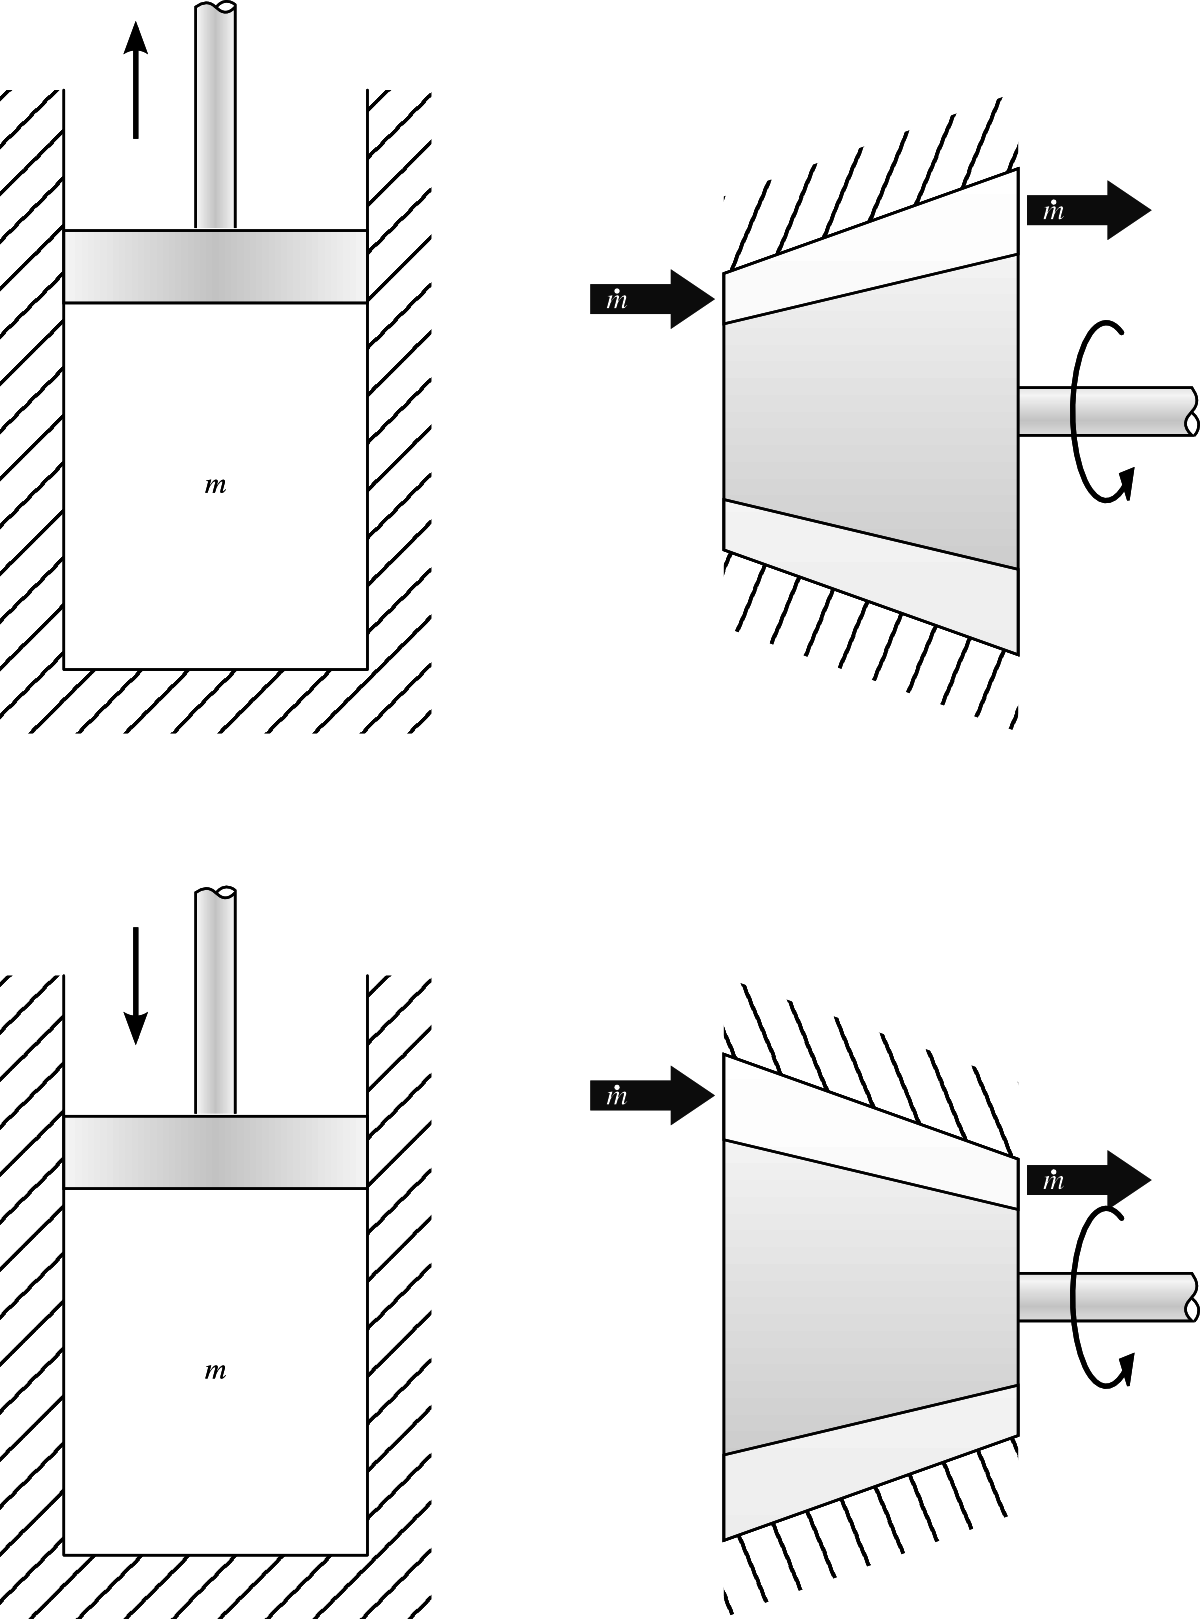
\includegraphics[width=8cm]{images/isentropique.png}
			\end{center}
			\supercaption{Évolution adiabatique réversible (isentropique) d’un gaz parfait. En système fermé (à gauche) comme en système ouvert (à droite), l’appareil est parfaitement isolé, de sorte qu’il n’y ait aucun transfert de chaleur, même si la température du gaz varie.}{\cczero \oc}
			\label{fig_gp_isentropique}
		\end{figure}
		
		Une évolution \vocab{adiabatique réversible} est effectuée infiniment lentement. Un piston dans un cylindre devra pour cela être déplacé infiniment lentement, et un compresseur en flux continu devra pour cela être infiniment long. Plus tard, dans le \courshuit, nous appellerons ces transformations \vocab{isentropiques}.

		\begin{figure}
			\begin{center}
				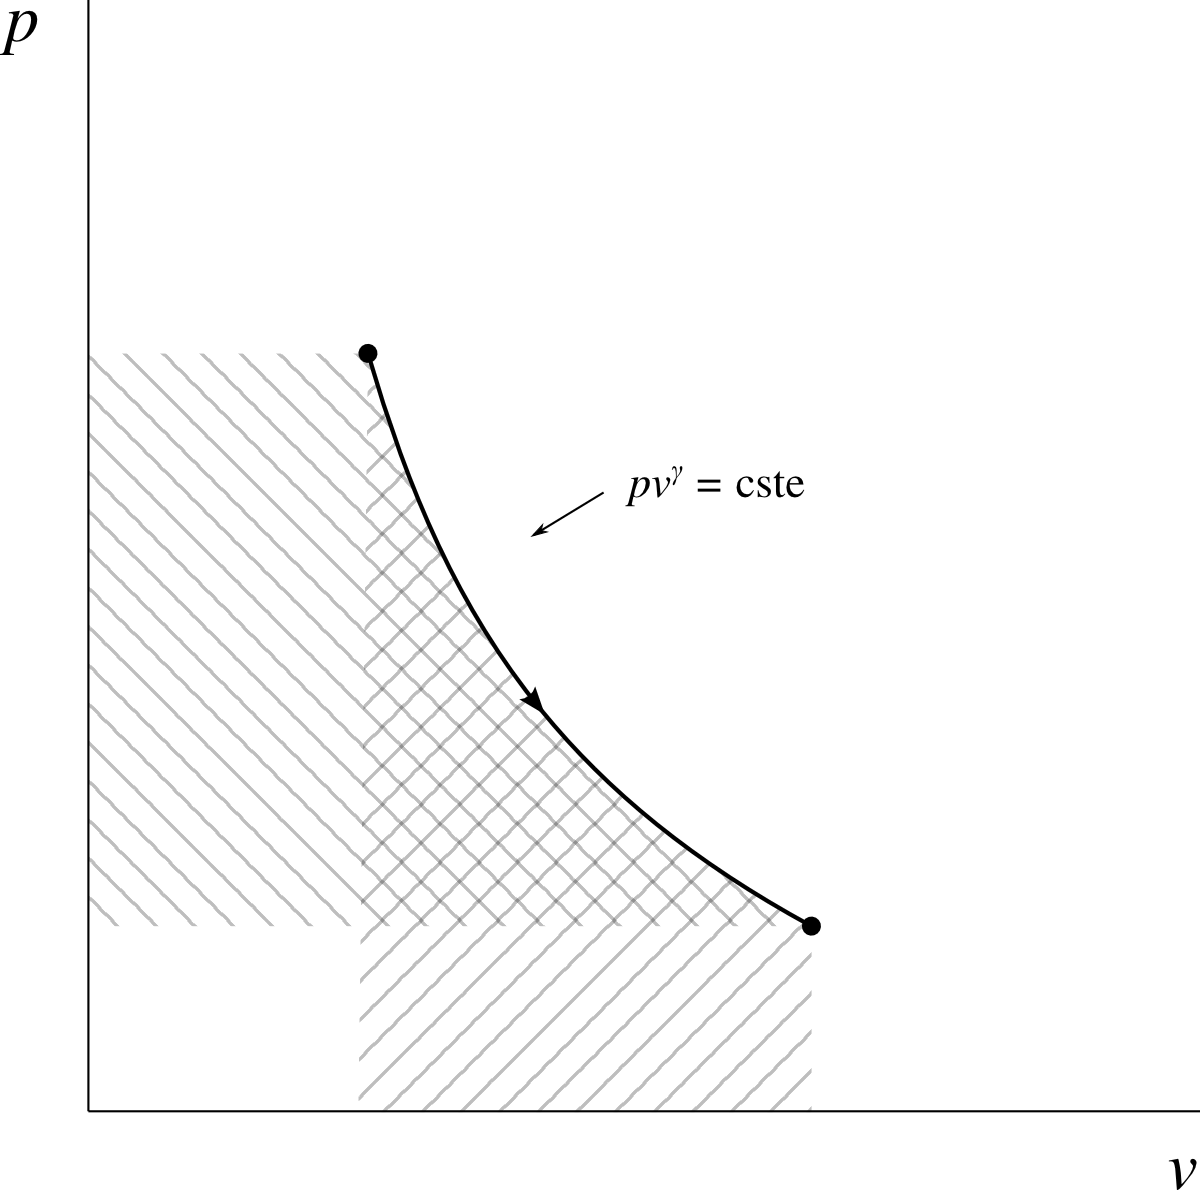
\includegraphics[width=\pvdiagramwidth]{images/pv_isentropique.png}
			\end{center}
			\supercaption{Détente adiabatique réversible d’un gaz parfait, représentée sur un diagramme pression-volume.}{\cczero \oc}
			\label{fig_gp_isentropique_pv}
		\end{figure}

		
		En système fermé, nous avons $q_{1\to2} + w_{1\to2} = \Delta u$ et, si l’évolution est réversible, la chaleur et le travail sont quantifiés sans la moindre difficulté :
		\begin{equation}
			q_{1\to2} = 0
		\end{equation}
		\begin{equationterms}
			\item lors d’une évolution adiabatique réversible, par définition.
		\end{equationterms}
		\begin{IEEEeqnarray}{rCl}
			w_{1\to2} 	& = & \Delta u - q_{1\to2} = \Delta u \nonumber \\
			w_{1 \to 2} 	& = & c_v \ \Delta T
			\label{eq_gp_travail_isentropique_sf}
		\end{IEEEeqnarray}
		\begin{equationterms}
			\item lors d’une évolution adiabatique réversible en système fermé.
		\end{equationterms}

		
		Lorsque l’évolution se fait en système ouvert, nous avons $q_{1\to2} + w_{1\to2} = \Delta h$ et nous pouvons de même écrire :
		\begin{IEEEeqnarray}{rCl}
			q_{1\to2} 	& = & 0 	\\
			w_{1\to2} 	& = & c_p \ \Delta T
			\label{eq_gp_travail_isentropique_so}
		\end{IEEEeqnarray}
		\begin{equationterms}
			\item lors d’une évolution adiabatique réversible, en système ouvert.
		\end{equationterms}

		
		Malheureusement, ces deux équations~\ref{eq_gp_travail_isentropique_sf} et~\ref{eq_gp_travail_isentropique_so} ne sont d’aucune utilité tant que l’on a pas prédit la température $T_2$ à la fin de l’évolution. Or, dans une évolution adiabatique réversible, rien ne reste constant : le volume spécifique, la pression et la température varient tous les trois. Comment quantifier ces propriétés ?
		
		
		Partons d’une évolution adiabatique infiniment courte dans un système fermé. Lorsque l’évolution est réversible, $\diff w = -p \diff v $ et alors :
		\begin{IEEEeqnarray*}{rCl}
			\diff q = \diff u - \diff w 	& = & 0		\nonumber \\
			\diff u + p \diff v				& = & 0
		\end{IEEEeqnarray*}

		Comme $\diff u = c_v \diff T$ pour un gaz parfait et que $p = R T/v $, on peut ré-écrire cette équation ainsi :
		\begin{IEEEeqnarray*}{rCl}
			c_v \diff T + \frac{R T}{v} \diff v								& = & 0	\nonumber \\
			\frac{1}{T} \diff T + \frac{R}{c_v} \frac{1}{v} \diff v 	& = & 0
		\end{IEEEeqnarray*}
	
		En intégrant entre deux états 1 et 2 :
		\begin{IEEEeqnarray}{rCl}
			\ln \left( \frac{T_2}{T_1} \right) + \frac{R}{c_v} \ln \left( \frac{v_2}{v_1} \right) 	& = & 0	\nonumber \\
			\ln \left( \frac{T_2}{T_1} \right) + \ln \left( \frac{v_2}{v_1} \right)^{\frac{R}{c_v}} 	& = & 0	\nonumber \\
			\ln \left( \frac{T_2}{T_1} \right) & = & \ln \left( \frac{v_1}{v_2} \right)^{\frac{R}{c_v}}
			\label{eq_tmp_isentropique}
		\end{IEEEeqnarray}
	
		Et comme $R = c_p-c_v$ (\ref{eq_sectionmathschiante_2}) et $\gamma \equiv c_p/c_v$ (\ref{def_gamma}), on a $\frac{R}{c_v} = \gamma -1$, ce qui permet de reformuler l’\cref{eq_tmp_isentropique} ci-dessus :
		\begin{equation*}
			\left( \frac{T_2}{T_1} \right) = \left(\frac{v_1}{v_2} \right)^{\gamma -1}
		\end{equation*}
	
		Nous avons donc lié température et volume spécifique lorsque l’évolution est adiabatique réversible (privée de transfert de chaleur et infiniment lente).

		Quelques manipulations algébriques, qu’il est laissé à l’étudiant/e le soin de réviser, nous permettent de décliner cette expression en fonction de la pression. On obtient ainsi les trois relations :
		\begin{IEEEeqnarray}{rCl}
			\left( \frac{T_1}{T_2} \right)	& = & \left( \frac{v_2}{v_1} \right)^{\gamma -1}		\label{eq_isentropique_horrible1}\\
			\left( \frac{T_1}{T_2} \right)	& = & \left( \frac{p_1}{p_2} \right)^{\frac{\gamma -1}{\gamma}}	\label{eq_isentropique_horrible2}\\
			\left( \frac{p_1}{p_2} \right)	& = & \left( \frac{v_2}{v_1} \right)^{\gamma}			\label{eq_isentropique_horrible3}
		\end{IEEEeqnarray}
		\begin{equationterms}
			\item pour toute évolution adiabatique réversible.
		\end{equationterms}

		Cette dernière \cref{eq_isentropique_horrible3} équivaut à l’expression :
		\begin{equation}
			p v^{\gamma} = \text{constante}
			\label{eq_isentropique_horrible3bis}
		\end{equation}
		\begin{equationterms}
			\item pour toute évolution adiabatique réversible.
		\end{equationterms}

		Nous disposons donc d’une relation simple entre pression et volume pour un gaz parfait suivant une évolution réversible adiabatique. Remarquons une dernière fois que, même si par définition aucune chaleur n’est transférée, la température varie systématiquement, comme l’indique la relation~\ref{eq_isentropique_horrible1}.
		
		\begin{anexample}
			Pour l’air, on mesure $c_{p\text{(air)}} = \SI{1005}{\joule\per\kilogram\per\kelvin}$, $c_{v\text{(air)}} = \SI{718}{\joule\per\kilogram\per\kelvin}$, $R_\text{air} = \SI{287}{\joule\per\kilogram\per\kelvin}$, et $\gamma_\text{air} = \num{1,4}$.\\
			Un réservoir d’air comprimé de~\SI{50}{\liter} contient de l’air à~\SI{40}{\bar} et~\SI{50}{\degreeCelsius}. L’atmosphère ambiante est à~\SI{1}{\bar}. Quelle est la quantité maximale de travail que l’on peut extraire de l’air comprimé sans lui fournir de chaleur ?
				\begin{answer}
					Le travail maximal sera obtenu si la détente est réversible. Comme nous ne pouvons pas apporter de chaleur, notre meilleure option est donc ici d’effectuer une détente adiabatique réversible depuis \SI{40}{\bar} jusqu’à \SI{1}{\bar}.\\
					Nous voulons calculer la température finale, car c’est elle qui nous donnera la variation d’énergie, donc le travail perdu par le gaz. Des trois intimidantes relations \ref{eq_isentropique_horrible1} à \ref{eq_isentropique_horrible3}, c’est la seconde qui nous intéresse : $\left( \frac{T_\A}{T_\B} \right)	= \left( \frac{p_\A}{p_\B} \right)^{\frac{\gamma -1}{\gamma}}$. Ainsi : $T_\B = T_\A \left( \frac{p_\A}{p_\B} \right)^{-\frac{\gamma -1}{\gamma}} = (\num{50} + \num{273,15}) \left( \frac{40}{1} \right)^{\frac{\num{1,4} -1}{\num{1,4}}} = \SI{112,6}{\kelvin} = \SI{-160,5}{\degreeCelsius}$.\\
					Le travail effectué par le système fermé constitué par le gaz est donc $w_\fromatob = \Delta u - q_\fromatob = c_v \ \Delta T - 0 = \num{718} \times (\num{-160,5} - \num{50}) = \SI{-1,5115e5}{\joule\per\kilogram} = \SI{-151,1}{\kilo\joule\per\kilogram}$.\\
					En calculant la masse $m_\A = \frac{p_\A V_\A}{R \ T_\A} = \frac{\num{40e5} \times \num{0,2}}{287 \times \ (\num{50} + \num{273,15})} = \SI{8,626}{\kilogram}$, nous obtenons $W_\fromatob = m_\A w_\fromatob = \num{8,626} \times \num{-151,1e3} = \SI{-1,3038e6}{\joule} = \SI{-1,304}{\mega\joule}$.
					\begin{remark} Cela représente suffisamment d’énergie pour accélérer sans frottement un véhicule de~\SI{1}{\tonne} jusqu’à une vitesse $C = \left[\frac{\num{1,3038e6}}{\frac{1}{2} \times \num{1000}}\right]^{\num{0,5}} = \SI{51,1}{\metre\per\second} \approx \SI[per-mode = symbol]{180}{\kilo\metre\per\hour}$.\end{remark}
					\begin{remark}La température finale, \SI{-160}{\degreeCelsius} (!), nous rappelle qu’il ne faut pas confondre «~adiabatique~» et «~à température constante~».\end{remark}
					\begin{remark}Les pressions peuvent être laissées en \si{bars} dans les fractions, mais les températures ne peuvent rester en~\si{\degreeCelsius}.\end{remark}
					\begin{remark}La détente correspond au maximum de travail car elle est réversible. Si elle ne l’était pas, alors la température du gaz chuterait moins et le travail serait plus faible (nous aurions toujours $w = c_v \Delta T$). Dans le cas le plus extrême, celui de la détente de Joule et Gay-Lussac (\S\ref{ch_principe_de_joule}), la température resterait fixe à~\SI{50}{\degreeCelsius} et aucun travail ne serait développé.\end{remark}
				\end{answer}
		\end{anexample}

		
	\subsection{Évolutions arbitraires}
	
		Il faut bien garder en tête que l’on peut en pratique faire évoluer les propriétés d’un gaz \emph{de n’importe quelle façon arbitraire} (\cref{fig_gp_pv_coeur}).
		
		\begin{figure}
			\begin{center}
				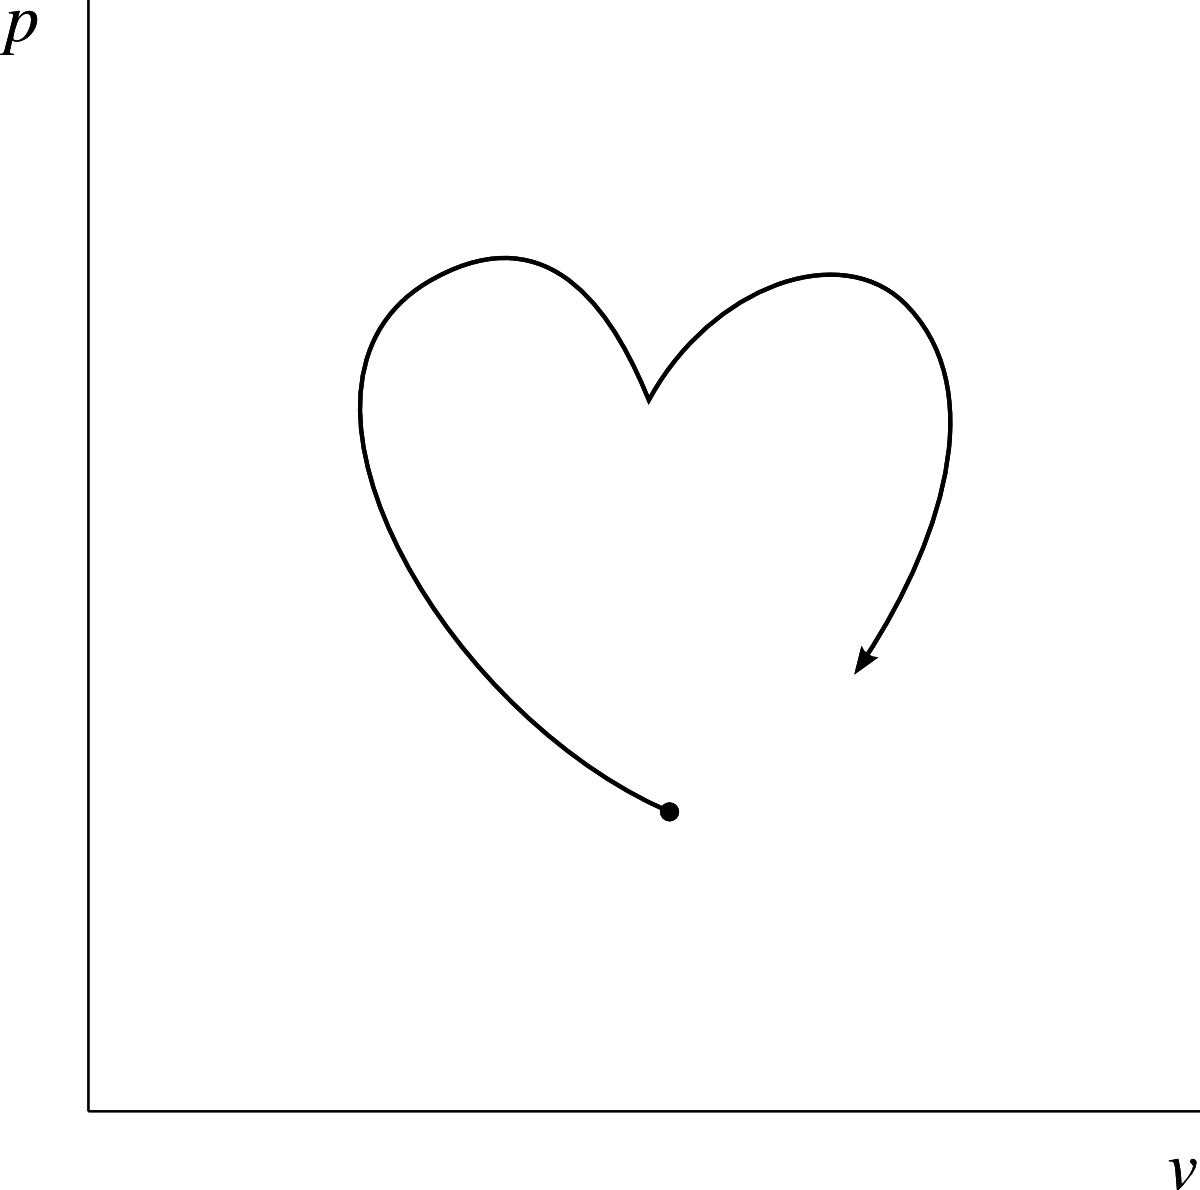
\includegraphics[width=\pvdiagramwidth]{images/pv_coeur.png}
			\end{center}
			\supercaption{Évolution entièrement arbitraire d’un gaz parfait représentée sur un diagramme pression-volume. Une telle évolution requiert une combinaison complexe de transferts de chaleur et de travail, que l’étudiant/e est invité/e à se représenter.}{\cczero \oc}
			\label{fig_gp_pv_coeur}
		\end{figure}
		
		Nous nous sommes concentrés sur quatre évolutions particulières des gaz parfaits, parce qu’elles jouent chacune un rôle important, pour les physiciens comme pour les ingénieur/es, dans la conception des machines thermiques. Cela ne doit toutefois pas limiter notre façon de «~penser~» un gaz et ses transformations. En contrôlant astucieusement les transferts de chaleur et de travail, nous pouvons bien sûr provoquer n’importe quelle évolution arbitraire.

\atstartofhistorysection
\onlyamphibook{\section[Un peu d’histoire : les questionnements de Lavoisier et Laplace]{Un peu d’histoire :\\ Lavoisier et Laplace s'interrogent sur la nature de la chaleur}}
\onlyframabook{\section[Un peu d’histoire : les questionnements de Lavoisier et Laplace]{Un peu d’histoire : Lavoisier et Laplace s'interrogent sur la nature de la chaleur}}
\label{ch_histoire_lavoisier_laplace_depondt}

\begin{center}\textit{Par Philippe Depondt\\ \begin{small}Université Pierre et Marie Curie, Paris\\ Contribution sous licence \ccbysa\end{small}}\end{center}

	Les débats sur la nature de la chaleur se sont poursuivis jusqu'à la fin du \textsc{xix}\ieme\ siècle avec l'acceptation progressive des théories atomiques. Une étape importante dans cette réflexion est fournie dans le \textit{Mémoire sur la chaleur} (1780~\cite{lavoisierlaplace1780}) de Lavoisier et Laplace :

	\begin{quote} «~Les physiciens sont partagés sur la nature de la chaleur. Plusieurs d’entre eux la regardent comme un fluide répandu dans toute la nature, et dont les corps sont plus ou moins pénétrés, à raison de leur température et de leur disposition particulière à le retenir ; il peut se combiner avec eux, et, dans cet état, il cesse d’agir sur le thermomètre et de se communiquer d’un corps à l’autre, ce n’est que dans l’état de liberté, qui lui permet de se mettre en équilibre dans les corps, qu’il forme ce que nous nommons chaleur libre. 

	D’autres physiciens pensent que la chaleur n’est que le résultat des mouvements insensibles des molécules de la matière. On sait que les corps, même les plus denses, sont remplis d’un grand nombre de pores ou de petits vides, dont le volume peut surpasser considérablement. celui de la matière qu’ils renferment ; ces espaces vides laissent à leurs parties insensibles la liberté d’osciller dans tous les sens, et il est naturel de penser que ces parties sont dans une agitation continuelle, qui, si elle augmente jusqu’à un certain point, peut les désunir et décomposer les corps ; c’est ce mouvement intestin qui, suivant les physiciens donc nous parlons, constitue la chaleur. 

	Pour développer cette hypothèse, nous ferons observer que, dans tous les mouvements dans lesquels il n’y a point de changement brusque, il existe une loi générale que les géomètres ont désignée sous le nom de principe de la conservation des forces vives ; cette loi consiste en ce que, dans un système de corps qui agissent les uns sur les autres d’une manière quelconque, la force vive, c’est-à-dire la somme des produits de chaque masse par le carré de sa vitesse, est constante. Si les corps sont animés par des forces accélératrices, la force vive est égale à ce qu’elle était à l’origine du mouvement, plus à la somme des masses multipliées par les carrés des vitesses dues à l’action des forces accélératrices. Dans l’hypothèse que nous examinons, la chaleur est la force vive qui résulte des mouvements insensibles des molécules d’un corps ; elle est la somme des produits de la masse de chaque molécule par le carré de sa vitesse. 

	Si l’on met en contact deux corps dont la température soit différente, les quantités de mouvements qu’ils se communiqueront réciproquement seront d’abord inégales ; la force vive du plus froid augmentera de la même quantité dont la force vive de l’autre diminuera, et cette augmentation aura lieu jusqu’à ce que les quantités de mouvement communiquées de part et d’autre soient égales ; dans cet état la température des corps sera parvenue à l’uniformité. 

	Cette manière d’envisager la chaleur explique facilement pourquoi l’impulsion directe des rayons solaires est inappréciable, tandis qu’ils produisent une grande chaleur. Leur impulsion est le produit de leur masse par leur simple vitesse ; or, quoique cette vitesse soit excessive, leur masse est si petite, que ce produit est presque nul, au lieu que leur force vive étant le produit de leur masse par le carré de leur vitesse, la chaleur qu’elle représente est d’un ordre très-supérieur à celui de leur impulsion directe. Cette impulsion sur un corps blanc, qui réfléchit abondamment la lumière, est plus grande que sur un corps noir, et cependant les rayons solaires communiquent au premier une moindre chaleur, parce que ces rayons, en se réfléchissant, emportent leur force vive, qu’ils communiquent au corps noir qui les absorbe. 

	Nous ne déciderons point entre les deux hypothèses précédentes ; plusieurs phénomènes paraissent favorables à la dernière ; tel est, par exemple, celui de la chaleur que produit le frottement de deux corps solides ; mais il en est d’autres qui s’expliquent plus simplement dans la première ; peut-être ont-elles lieu toutes deux à la fois. Quoi qu’il en soit, comme on ne peut former que ces deux hypothèses sur la nature de la chaleur, on doit admettre les principes qui leur sont communs ; or, suivant l’une et l’autre, la quantité de chaleur libre reste toujours la même dans le simple mélange des corps. Cela est évident, si la chaleur est un fluide qui tend à se mettre en équilibre, et, si elle n’est que la force vive qui résulte du mouvement intestin de la matière, le principe dont il s’agit est une suite de celui de la conservation des forces vives. La conservation de la chaleur libre, dans le simple mélange des corps, est donc indépendante de toute hypothèse sur la nature de la chaleur ; elle a été généralement admise par les physiciens, et nous l’adopterons dans les recherches suivantes.~» \end{quote} 

	À l'époque où ce texte a été écrit, l'hypothèse atomique restait largement spéculative, faute de moyens expérimentaux adéquats : l'expérience de Jean Perrin qui a finalement tranché n'a eu lieu que dans les premières années du \textsc{xx}\ieme\ siècle et les expériences de diffraction de rayons X suggérées par Max von Laue en 1912. 

\atendofhistorysection


\atstartofexercices
	\begin{boiboiboite}
	\propair
	\isentropiques
	\isothermes
\end{boiboiboite}

% idea: aircraft tyre deflation after MERTO

\subsubsection{Pression d’air}
\label{exo_pression_air}

	Une masse de~\SI{5}{\kilogram} d’air est enclose dans un réservoir de~\SI{2}{\metre\cubed}.

	\begin{enumerate}
		\item Quelles sont son volume spécifique et sa masse volumique ?
		\item Quelle est la pression si la température est de~\SI{20}{\degreeCelsius} ?
	\end{enumerate}
	
\subsubsection{Réchauffement d’un réservoir d’air}
\label{exo_rechauffement_reservoir_air}
\wherefrom{dérivé du rattrapage S1 2013}% reconstruit à partir du rattrapage 20130621

	Un réservoir hermétique d’air comprimé en béton a un volume fixe de~\SI{1,2}{\metre\cubed}. L’air y est stocké à pression de~\SI{2}{\bar}. \\
	Le réservoir est placé au soleil et le réchauffement solaire fait passer la température de~\SI{5}{\degreeCelsius} à~\SI{60}{\degreeCelsius}.
	
	\begin{enumerate}
		\item Quelles sont la masse, le volume spécifique, la masse volumique et la pression à l’intérieur du réservoir, avant et après le réchauffage ?
	\end{enumerate}

	Lorsque la température atteint~\SI{60}{\degreeCelsius}, une soupape s’ouvre et laisse de l’air s’échapper pour faire redescendre la pression dans le réservoir jusqu’à la pression initiale de~\SI{2}{\bar}. Pendant l’échappement, la température de l’air à l’intérieur du réservoir reste constante.

	\begin{enumerate}
		\shift{1}
		\item Quelle masse d’air doit-on laisser échapper ?
	\end{enumerate}

	Lorsque la pression a atteint~\SI{2}{\bar}, la soupape se referme et le réservoir, de nouveau hermétique, se refroidit lentement à volume constant. La température finale revient à~\SI{5}{\degreeCelsius}.
	
	\begin{enumerate}
		\shift{2}
		\item Quelle est la pression finale dans le réservoir ?
	\end{enumerate}


\subsubsection{Énergie et température}
\label{exo_gp_energie_temperature}

	De l’air dans un compartiment flexible est à pression de~\SI{3}{\bar}. Son énergie interne est de~\SI{836}{\kilo\joule\per\kilogram}.
	
	Il est chauffé à pression constante jusqu’à~\SI{900}{\degreeCelsius} ; il est ensuite refroidi et détendu alors que ses propriétés varient selon la relation $p v^{\num{1.1}} = \text{cste.}$ jusqu’à ce que sa température atteigne~\SI{25}{\degreeCelsius}.

	\textit{[Question piège]} Combien d’énergie a-t-il reçu ou perdu depuis le début de l’évolution ?

\subsubsection{Puissance d’une pompe à air}
\label{exo_puissance_pompe_air}

	Une pompe à air (\cref{fig_exo_compresseur_air}) comprime de l’air en régime permanent, de façon adiabatique. L’air voit sa température augmenter de~\SI{15}{\degreeCelsius} à~\SI{100}{\degreeCelsius}.
	
	Quelle est la puissance spécifique consommée ?

	\begin{figure}[!bh]
		\begin{center}
			\onlyframabook{\vspace{-0.3cm}}%handmade
			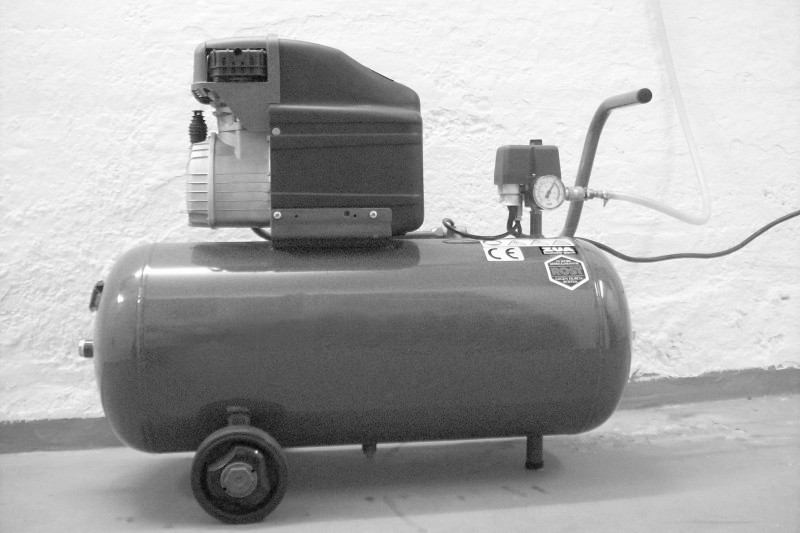
\includegraphics[width=0.6\columnwidth]{images/compresseur_air_reservoir.jpg}
			\onlyframabook{\vspace{-0.6cm}}%handmade
		\end{center}
		\supercaption{Un petit compresseur électrique monté sur un réservoir d’air portatif}{\wcfile{Kolbenkompressor.jpg}{Photo} par \wcu{Grikalmis} (retouchée, \pd)}
		\label{fig_exo_compresseur_air}
	\end{figure}

\onlyframabook{\vspace{-1em}}	
\onlyamphibook{\par~\clearfloats\dontbreakpage}%handmade
\subsubsection{Turbine de turboréacteur}
\label{exo_gp_turbine_turboreacteur}
\wherefrom{[DS n°2 2011, 3pts]}
	
	Un/e étudiant/e démonte le turboréacteur \textit{\wf{Turbomeca Marboré}} d’un \wfd{Fouga CM-170 Magister}{Fouga Magister} pour en étudier et en modifier le fonctionnement. Il/elle fait fonctionner le moteur sur un banc d’essai.
	
	À l’entrée de la turbine, les conditions sont mesurées à~\SI{110}{\metre\per\second} et~\SI{1000 }{\degreeCelsius} .\\
	À la sortie de la turbine, ces propriétés sont mesurées à~\SI{125}{\metre\per\second} et~\SI{650}{\degreeCelsius} .
	
	L’étudiant/e mesure également les pertes sous forme de chaleur de la turbine : \SI{75}{\kilo\joule\per\kilogram}.
	
	\begin{enumerate}
		\item Quelle est la puissance mécanique spécifique développée par la turbine ?
		\item Quelle condition l’étudiant/e doit-il/elle maintenir pour obtenir une puissance de~\SI{1}{\mega\watt} ?
	\end{enumerate}


\subsubsection{Évolutions élémentaires : compression isotherme}
\label{exo_gp_isotherme}
\wherefrom{[DS n°2 2011, 4pts]}
% Cet exo est lié à l’exercice 8.5 (\ref{exo_diagrammes_ts})

	Une masse de~\SI{3,5}{\kilogram} d’air est comprimée de façon réversible isotherme (à température constante) depuis~\SI{2}{\bar} et~\SI{15}{\degreeCelsius} jusqu’à~\SI{45}{\bar}.
	
	\begin{enumerate}
		\item Représentez l’évolution sur un diagramme pression-volume, de façon qualitative (c’est-à-dire sans représenter les valeurs numériques).
		\item Quelles sont les quantités de travail et de chaleur mises en jeu ?
		\item Si la compression était effectuée de façon adiabatique réversible, le volume final serait-il différent ?
	\end{enumerate}
	

\subsubsection{Évolutions élémentaires : refroidissements isobare et isochore}
\label{exo_gp_isobare_isochore}
\wherefrom{[DS n°2 2010, 5pts]}
% Cet exo est lié à l’exercice 8.5 (\ref{exo_diagrammes_ts})

	Une masse de~\SI{2}{\kilogram} d’air dans un réservoir déformable est à pression de~\SI{4,5}{\bar} et occupe un volume de~\SI{800}{\liter}. Elle est refroidie et le réservoir maintient la pression constante jusqu’à ce que le volume ait été réduit de~\SI{40}{\percent}.
	
	Ensuite, le refroidissement est continué à volume constant jusqu’à ce que la température atteigne~\SI{25}{\degreeCelsius}.
	
	\begin{enumerate}
		\item Tracez l’évolution suivie sur un diagramme pression-volume.
		\item Quel est le travail effectué par l’air ?
		\item Quel est le coût total en chaleur pour la totalité de l’évolution ?
	\end{enumerate}


\subsubsection{Évolutions élémentaires : compression isentropique}
\label{exo_gp_isentropique}
	
	Quelle quantité minimale de travail faut-il pour comprimer~\SI{5}{\kilogram} d’air à~\SI{1}{\bar} et~\SI{20}{\degreeCelsius} jusqu’à \SI{50}{\bar} sans transfert de chaleur ? Tracez l’évolution suivie par l’air sur un diagramme pression-volume.


\subsubsection{Évolutions élémentaires : vocabulaire}
\label{exo_bete_mechant}
\wherefrom{[DS n°2 2010, 2pts]}

	Une masse fixe de gaz parfait, avec pour seul espoir de contrarier un/e étudiant/e en thermodynamique, suit lentement les évolutions suivantes :

		\begin{center}
			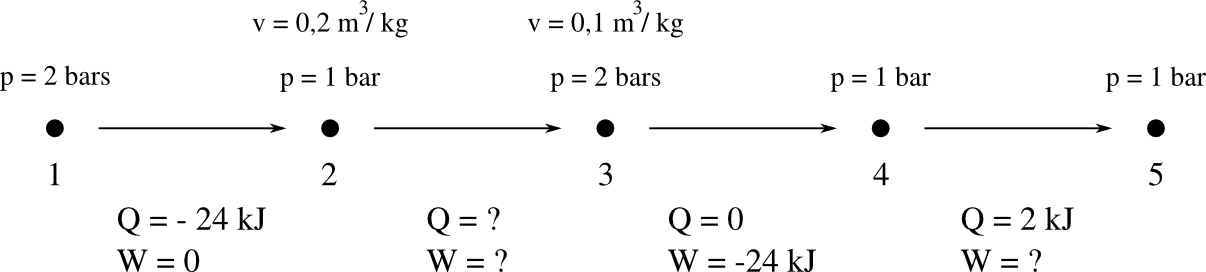
\includegraphics[width=\textwidth]{images/exo_elementaires.png}
		\end{center}

	Parmi les évolutions ci-dessus, lesquelles sont :
	\begin{enumerate}
		\item à température constante (isotherme) ?
		\item à volume constant (isochore) ?
	\end{enumerate}


\subsubsection{Évolutions élémentaires : pression et volume}
\label{exo_retrouver_pv}
\wherefrom{Partiel S1 2013, 2pts}

	Parmi les évolutions réversibles décrites sur chacun des graphiques de la \cref{fig_pvel}, identifiez (sans devoir vous justifier) l’évolution à température constante, à pression constante, adiabatique réversible, et à volume constant.
	
	\begin{figure}[!bh]
		\begin{center}
			%\vspace{-0.1cm}%handmade
			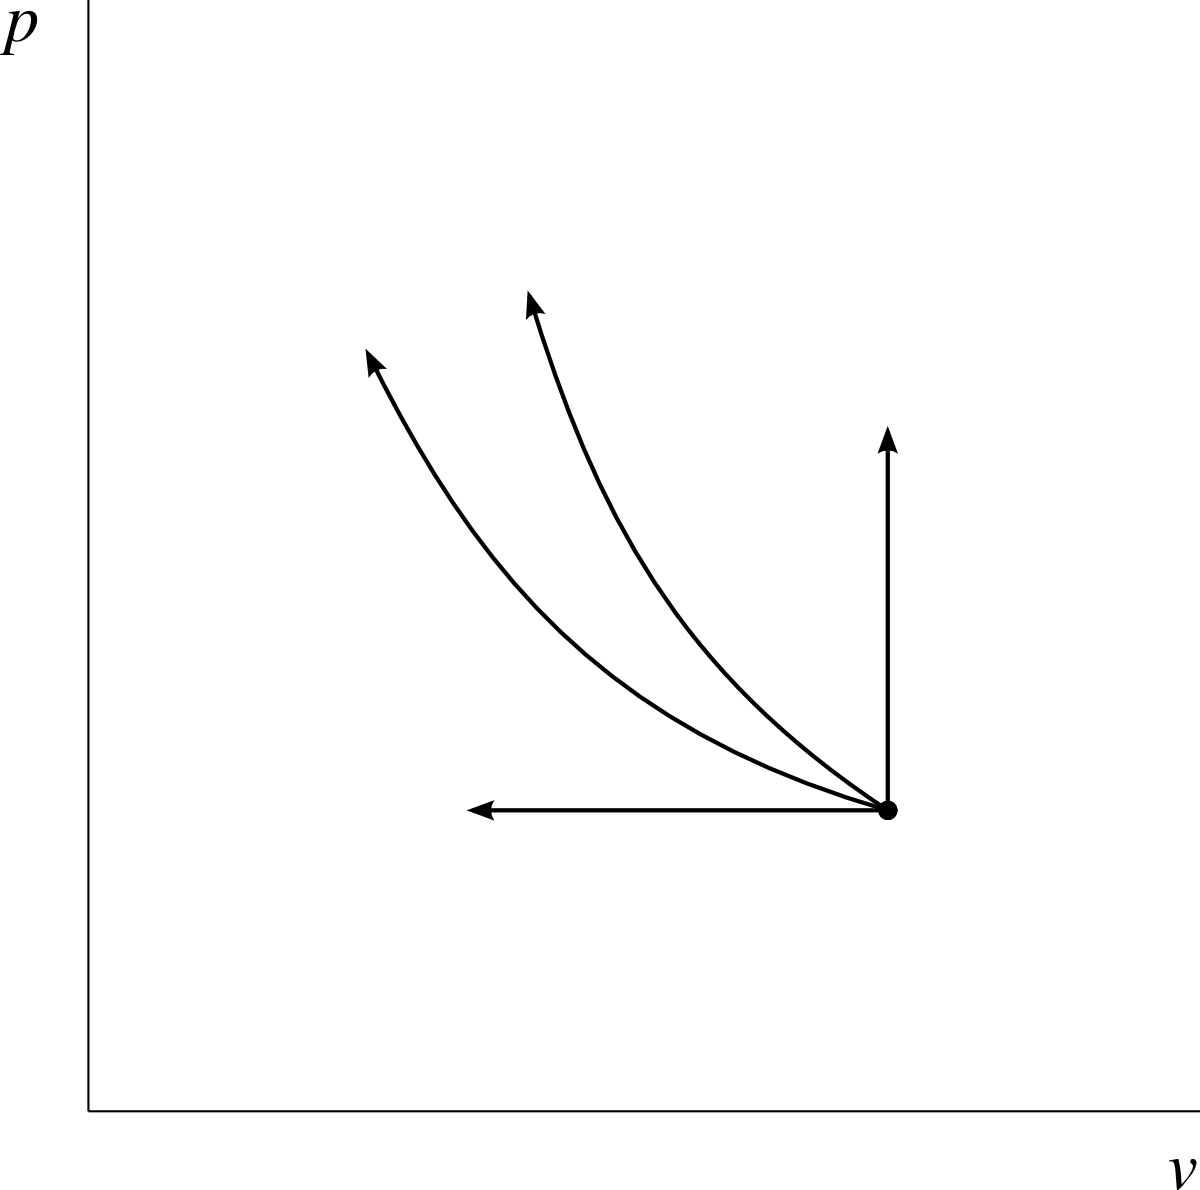
\includegraphics[width=0.4\textwidth, max width=0.6\columnwidth]{images/exo_pv_elementaires1.png}
			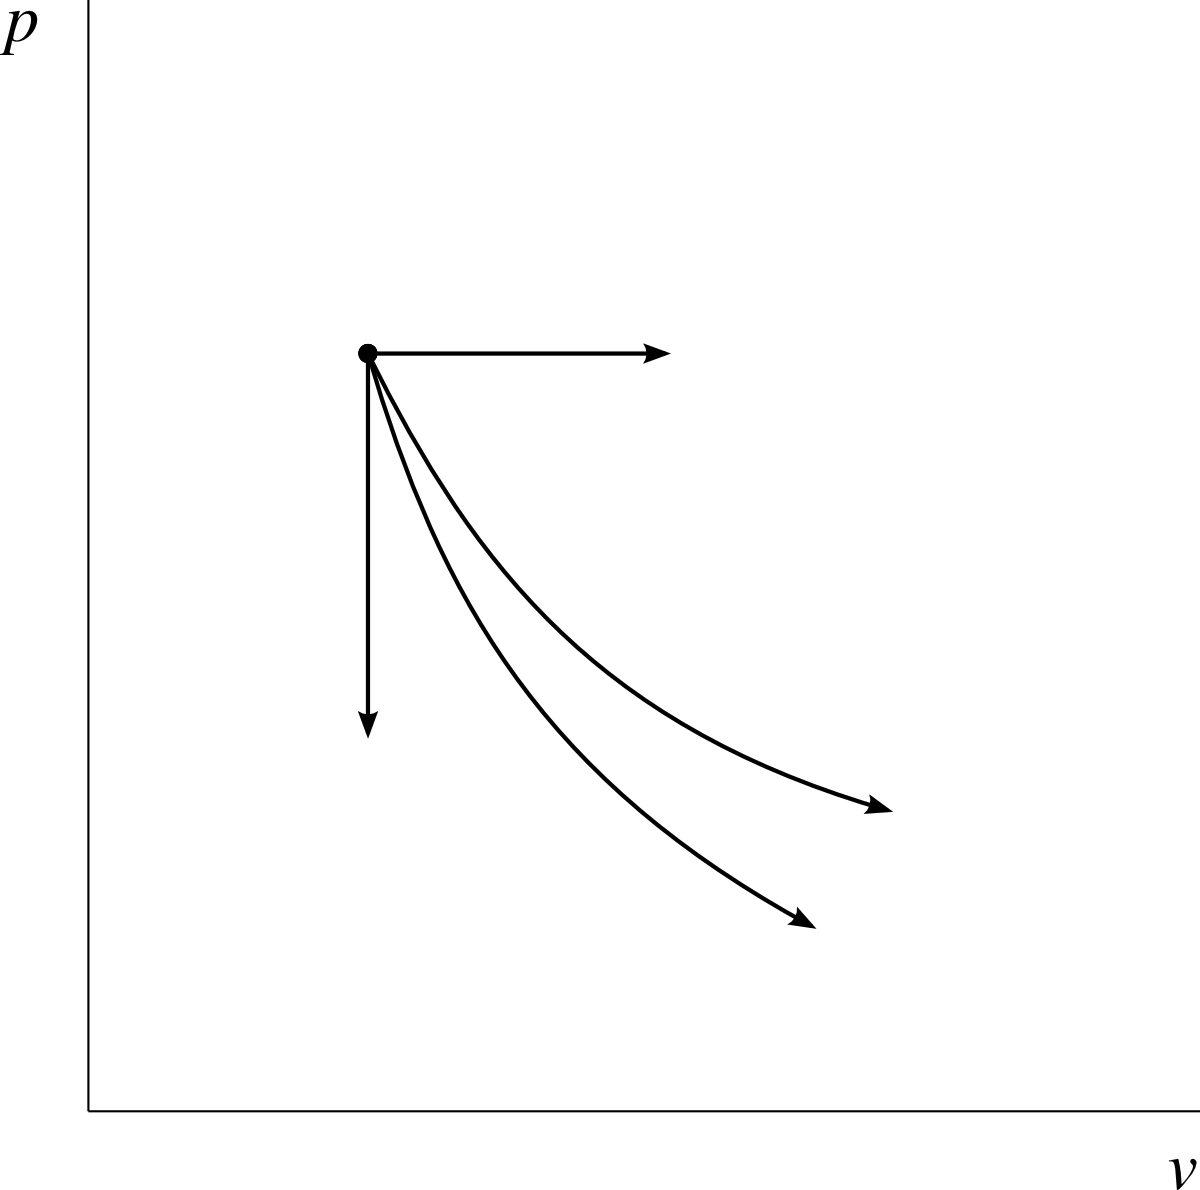
\includegraphics[width=0.4\textwidth, max width=0.6\columnwidth]{images/exo_pv_elementaires2.png}
			%\vspace{-0.1cm}%handmade
		\end{center}
		\supercaption{Évolutions élémentaires d’un gaz parfait}{schéma \cczero \oc}
		\label{fig_pvel}
	\end{figure}
	

\subsubsection{Compresseur de turboréacteur}
\label{exo_compresseur_turboreacteur}
\wherefrom{[Partiel S1 2012, 8pts]}

	À l’intérieur d’un des moteurs d’un avion de ligne, le compresseur (\cref{fig_exo_entree_genx2b}) est quasiment adiabatique.	
	
	\onlyamphibook{\begin{figure}[bh]}
	\onlyframabook{\begin{figure}[h!]}
		\begin{center}
			\onlyamphibook{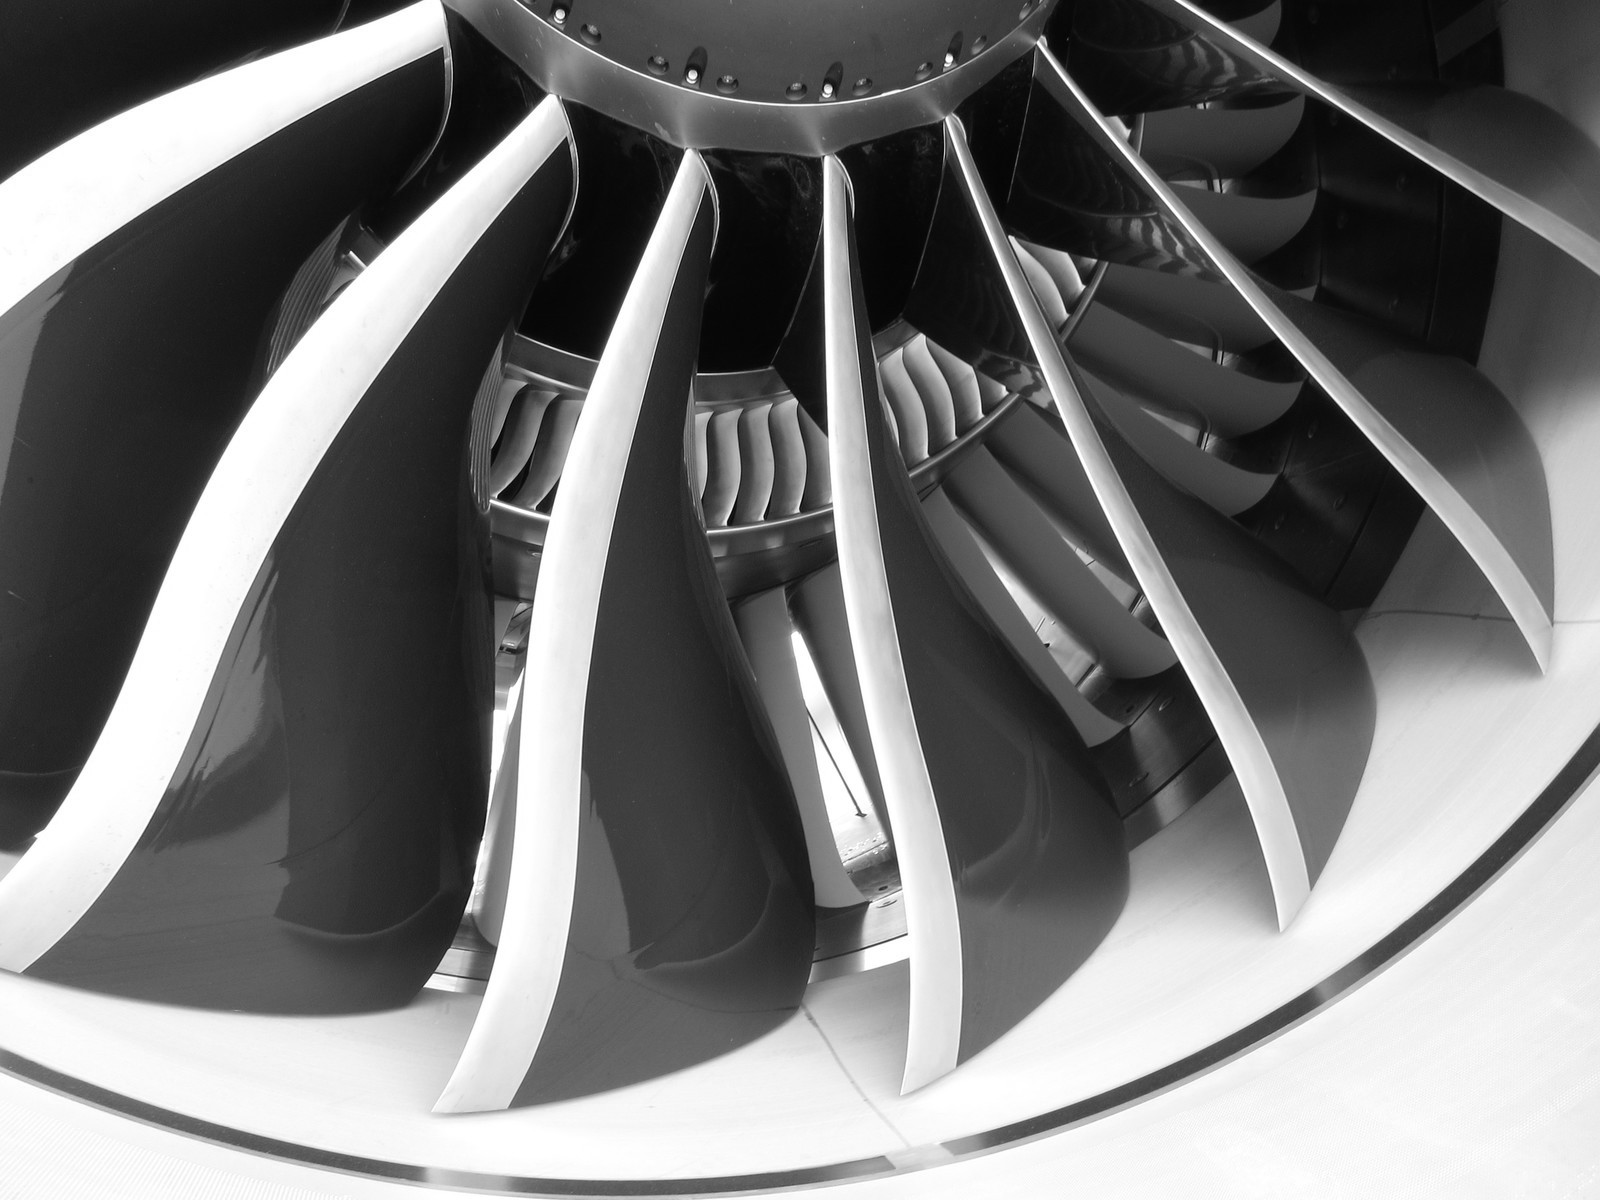
\includegraphics[width=0.8\textwidth]{images/entree_genx2b.jpg}}
			\onlyframabook{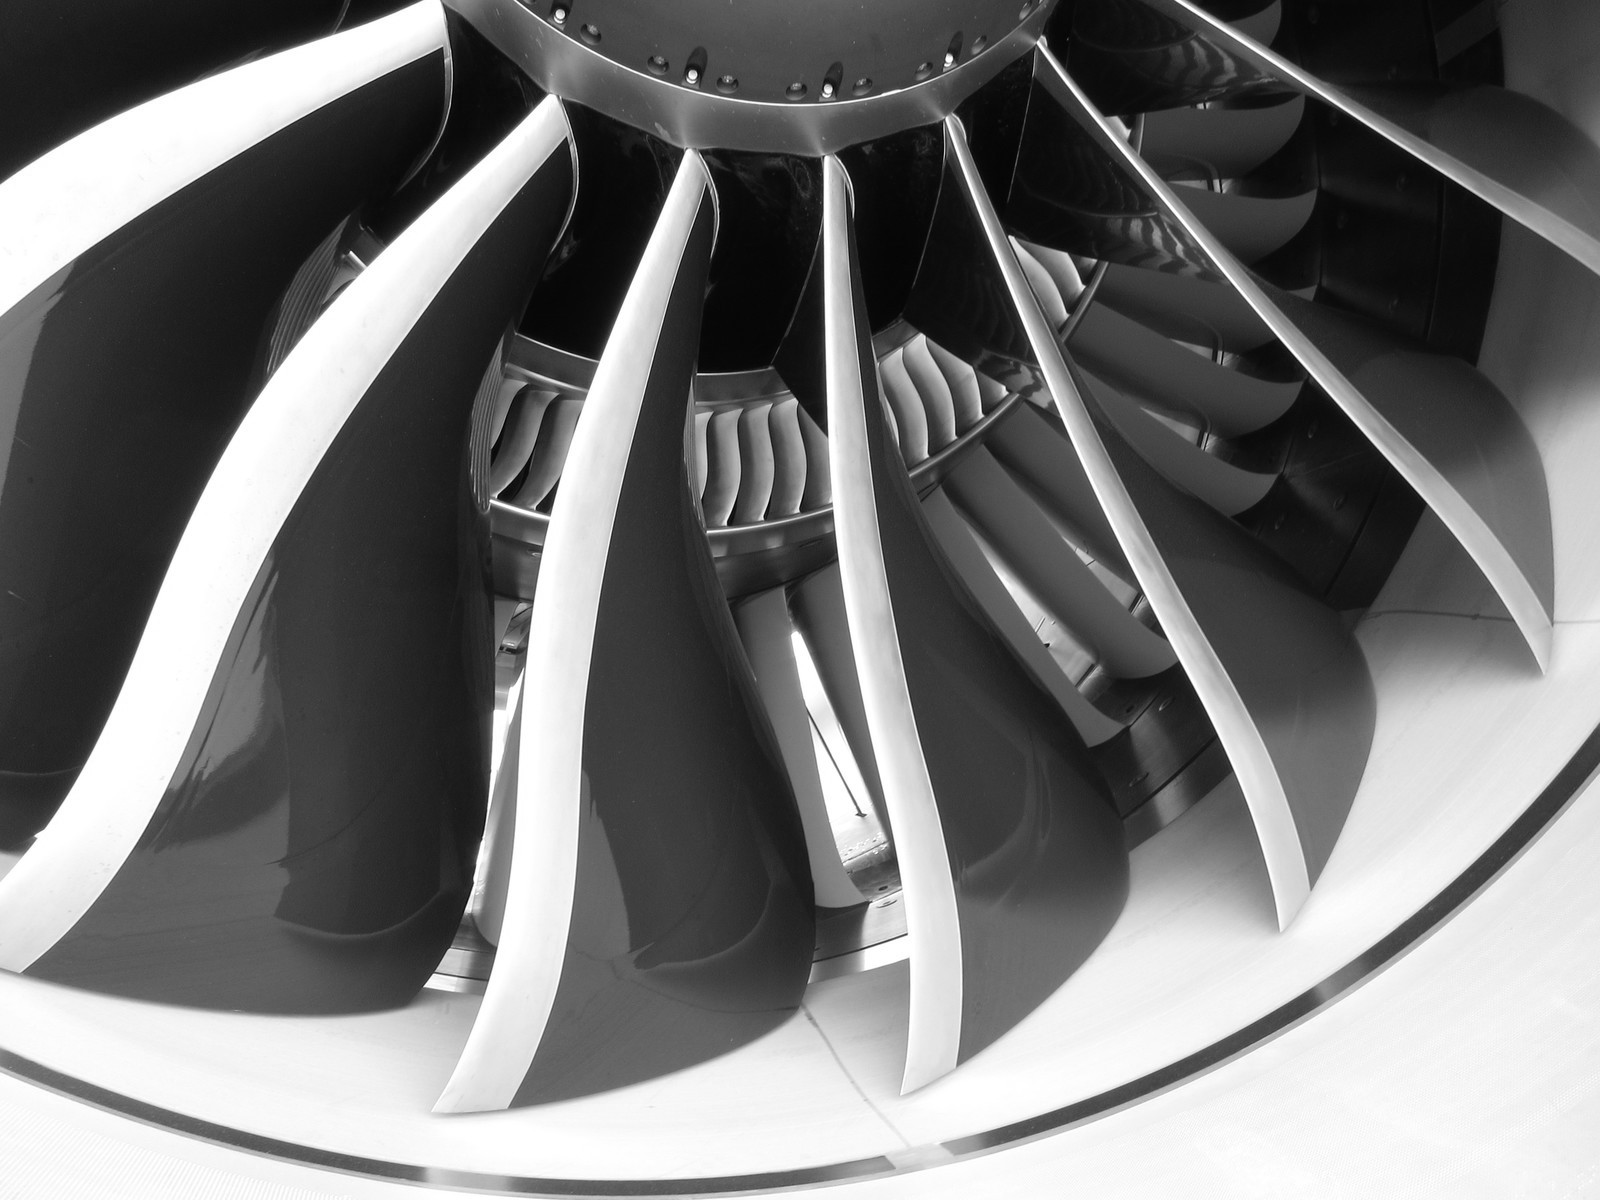
\includegraphics[width=0.9\columnwidth]{images/entree_genx2b.jpg}}
		\end{center}
		\supercaption{Entrée d’air d’un des quatre turboréacteurs General Electric \textsc{GEnx}-2B équipant un Boeing 747-8. Les pales bicolores de la soufflante sont visibles au premier plan ; derrière, le flux d’air est divisé entre l’entrée du compresseur (intérieur) et les stators redresseurs du flux froid (extérieur). }{Photo \ccbysa \olivier}
		\label{fig_exo_entree_genx2b}
	\end{figure}

	Pendant la croisière (atmosphère : \SI{33 000}{ft} ; \SI{-50}{\degreeCelsius} ; \SI{0,25}{\bar}), le compresseur est entraîné par la turbine par le biais d’un arbre mécanique. Il reçoit~\SI{55}{\kilogram\per\second} d’air aux conditions atmosphériques, qu’il compresse jusqu’à une pression de~\SI{8}{\bar}.
	% débit de masse : 1 Trent 500 au décollage = 1000 kg/s (source "the Jet Engine" Rolls-Royce plc 2005), estimé moitié moins en croisière soit 500 kg/s. Avec taux de dillution de 9 (pour le GEnx-2B en photo) on obtient ~ 55 kg/s.
	
	\begin{enumerate}
		\item À partir de la relation suivante,
			\begin{equation}
				\left( \frac{p_1}{p_2} \right)	= \left( \frac{v_2}{v_1} \right)^{\gamma} \tag{\ref{eq_isentropique_horrible3}}
			\end{equation}
			valable pour une évolution adiabatique réversible d’un gaz parfait, montrez (sans utiliser l’\cref{eq_isentropique_horrible1}) que :			
			\begin{equation}
				\left( \frac{T_1}{T_2} \right)	=  \left( \frac{p_1}{p_2} \right)^{\frac{\gamma -1}{\gamma}}  \tag{\ref{eq_isentropique_horrible2}}
			\end{equation}
		\item Quelle est la puissance minimale théorique à fournir au compresseur ?
		\item À quelles conditions obtiendrait-on cette puissance ?
	\end{enumerate}
	
	En réalité, le compresseur demande une puissance sensiblement plus grande pour fonctionner. Nous modélisons l’évolution réelle au sein du compresseur par deux phases distinctes :

	\begin{itemize}
		\item Un réchauffement à pression constante, effectué par frottement, avec une puissance représentant~\SI{15}{\percent} de la puissance mécanique théorique calculée plus haut ;
		\item Puis, une compression idéale jusqu’à~\SI{8}{\bar}.
	\end{itemize}
	
	\begin{enumerate}
		\shift{3}
		\item Comparez la compression théorique de la question 2 et cette nouvelle évolution sur un diagramme pression-volume. Représentez-y graphiquement le travail consommé sur l’une des évolutions.
		\item Quelle est la puissance consommée par le compresseur dans ce nouveau cas de figure ?
	\end{enumerate}


\subsubsection{Compression et combustion au sein d’un moteur Diesel}
\label{exo_compression_combustion_diesel}
\wherefrom{Partiel S1 2012, 8pts}
\index{Diesel!moteur}\index{Diesel!Rudolf}

	En 1890 un jeune ingénieur allemand épris de thermodynamique (\S\ref{ch_histoire_diesel}) met au point un moteur de faible puissance, faible vitesse et haute efficacité dans un laboratoire (\cref{fig_exo_moteur_diesel}). Le moteur se veut robuste et simple ; il n’a qu’un cylindre. Nous étudions ici une partie de son cycle de fonctionnement. %why not more?
	
	\begin{figure}
		\begin{center}
			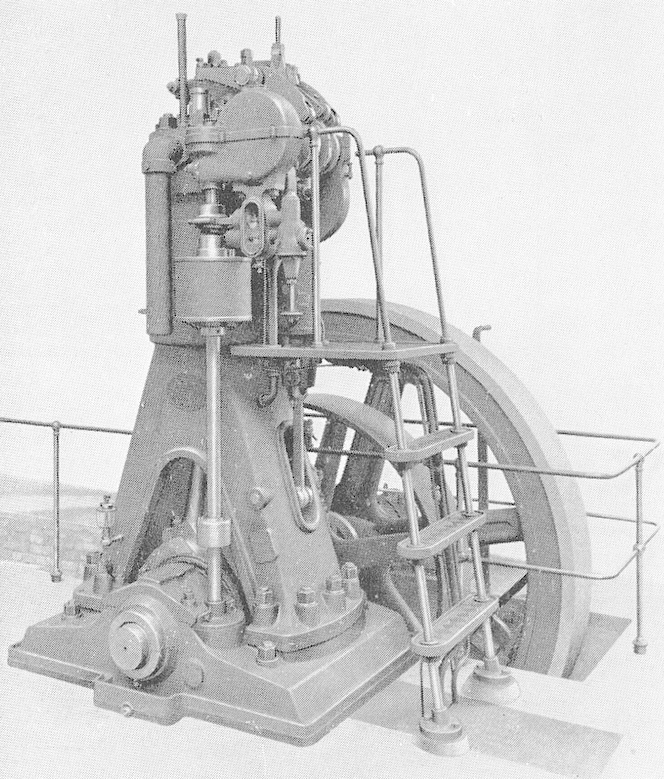
\includegraphics[width=0.5\textwidth]{images/Dieselmotor_1898_retouched.jpg}
		\end{center}
		\supercaption{Moteur Diesel de 1898, fabriqué sous licence par Sulzer en Suisse}{\wcfile{Dieselmotor 1898 (retouched).jpg}{Photo} \ccbysa Sulzer AG}
		\label{fig_exo_moteur_diesel}
	\end{figure}
	
	Le piston au sein du cylindre fait varier périodiquement le volume entre~\SI{3}{\liter} (\vocab{point mort bas}, piston en bas de sa course) et~\SI{0,3}{\liter} (\vocab{point mort haut}, piston en haut de sa course).
	
	Le moteur débute son cycle au point mort bas, alors qu’il est empli d’air à~\SI{20}{\degreeCelsius} et~\SI{1}{\bar}. Le piston comprime cet air jusqu’au point mort haut.
	
	La compression se fait de façon réversible (très lente), mais non-adiabatique : l’air reçoit de la chaleur au travers des parois tout au long de l’évolution. L’ingénieur prédit que ses propriétés varieront selon la relation $p \ v^{1,5} = \text{constante}$.


	\begin{enumerate}
		\item Le travail effectué par une force $\vec F$ sur un déplacement $\vec l$ s’exprime selon
			\begin{equation}
				W \equiv \vec F \cdot \vec l 	\tag{\ref{eq_travail_fdl}}
			\end{equation}
			À partir de cette équation, exprimez le travail effectué sur un corps de masse fixe en fonction de son volume spécifique et de sa pression interne.
		\item Combien d’énergie sous forme de travail la compression du gaz aura-t-elle coûté ?
		\item Combien d’énergie sous forme de chaleur le gaz aura-t-il reçu pendant la compression ?
	\end{enumerate}

	Lorsque le piston est arrivé en haut de sa course, on procède à l’injection progressive de carburant dans le cylindre pour permettre la combustion. La quantité de carburant injectée permet un apport total de chaleur de~\SI{2}{\kilo\joule}. La combustion se déroule à pression constante.
	
	\begin{enumerate}
		\shift{3}
		\item Représentez l’évolution suivie par le gaz pendant la compression et la combustion sur un diagramme pression-volume, de façon qualitative (c’est-à-dire sans représenter les valeurs numériques).
		\item Quelle sera la température maximale atteinte au sein du moteur ?
		\item Pour éviter une défaillance structurelle, l’ingénieur doit s’assurer que la force transmise par le piston n’excède jamais~\SI{10}{\kilo\newton}. Quelle contrainte doit-il respecter pour cela ?
	\end{enumerate}
	

\subsubsection{Turboréacteur simple flux}
\label{exo_turboreacteur_simple_flux}
\wherefrom{Partiel S1 2013, 10pts}
\index{turboréacteur}

	Un avion militaire des années 1960 est équipé d’un turboréacteur simple flux (\cref{fig_exo_turbojet}). Nous souhaitons calculer la vitesse maximale théorique à laquelle il pourrait accélérer l’air en sortie de tuyère.
	
	\begin{figure}
		\begin{center}
			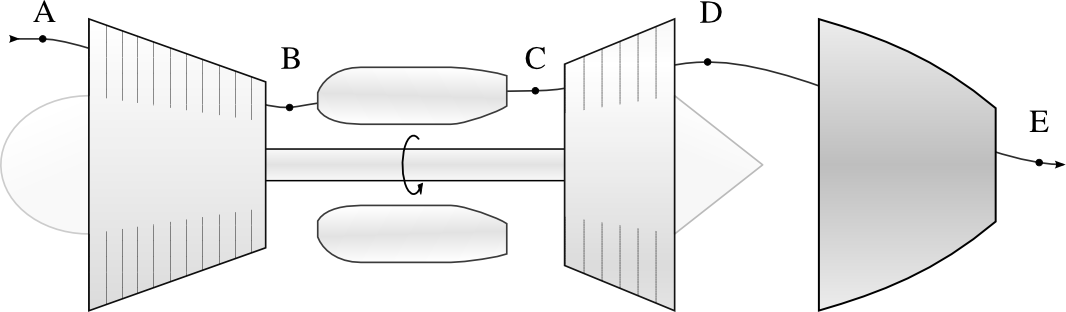
\includegraphics[width=\textwidth]{images/turbojet.png}
		\end{center}
		\supercaption{Schéma de principe d’un turboréacteur. L’air traverse la machine de gauche à droite.}{\ccbysa \olivier}
		\label{fig_exo_turbojet}
	\end{figure}
	
	Le moteur est testé sur un banc d’essai, à l’immobile. Lorsque l’air passe dans le turboréacteur, il traverse quatre composants que nous modéliserons comme s’ils étaient idéaux :
	
	\begin{description}
		\item [Le compresseur] (\cref{fig_exo_compresseur_turbojet}) comprime l’air de façon adiabatique réversible.\\
			À l’entrée, l’air est à~\SI{0,9}{\bar} et~\SI{5}{\degreeCelsius} ; à la sortie la pression est portée à~\SI{19}{\bar}.
		\item [La chambre de combustion] permet d’effectuer un réchauffement de l’air en maintenant sa pression constante.\\
			À la sortie de la chambre de combustion, la température a été portée à~\SI{1100}{\degreeCelsius}.
		\item [La turbine] extrait de l’énergie de l’air pour pouvoir alimenter le compresseur. Dans la turbine, l’air est détendu de façon adiabatique réversible.
		\item [La tuyère] est un composant dans lequel aucune puissance n’est apportée ni prélevée à l’air. Lorsqu’il la traverse, l’air se détend de façon adiabatique réversible ; sa vitesse augmente fortement. À la sortie de la tuyère, il a retrouvé la pression atmosphérique et est rejeté dans l’atmosphère.
	\end{description}
	
	Le but de l’exercice est de calculer la vitesse à laquelle le turboréacteur est capable de repousser l’air qu’il admet.
	
	\pagebreak[1] %handmade
	
	\begin{enumerate}
		\item À partir de la relation suivante,
			\begin{equation}
				\left( \frac{T_1}{T_2} \right)	= \left( \frac{v_2}{v_1} \right)^{\gamma -1} \tag{\ref{eq_isentropique_horrible1}}
			\end{equation}
			valable pour une évolution adiabatique réversible d’un gaz parfait, montrez (sans utiliser l’équation~\ref{eq_isentropique_horrible3}) que :			
			\begin{equation}
				\left( \frac{T_1}{T_2} \right)	=  \left( \frac{p_1}{p_2} \right)^{\frac{\gamma -1}{\gamma}} \tag{\ref{eq_isentropique_horrible2}}
			\end{equation}
		\item Quelle est la température de l’air à la sortie du compresseur ?
		\item Quelle est ainsi la puissance spécifique consommée par le compresseur ?
		\item Quelle est la puissance spécifique apportée sous forme de chaleur dans la chambre de combustion ?
		\item Quelle doit être la température à la sortie de la turbine pour qu’elle puisse alimenter le compresseur ?
		\item Quelle sera alors la pression à la sortie de la turbine ?
		\item Quelle sera la température des gaz d’échappement, à la sortie de la tuyère ?
		\item Quelle sera enfin la vitesse d’éjection des gaz à la sortie de la tuyère ?
		\item Représentez l’évolution sur un diagramme pression-volume, de façon qualitative.
		\item Sur le même diagramme pression-volume, tracez l’évolution qui serait suivie par le gaz si le compresseur ne pouvait pas effectuer une compression réversible (compresseur réel, compression avec frottement interne).
	\end{enumerate}

	
	\begin{figure}[bth]
		\begin{center}
			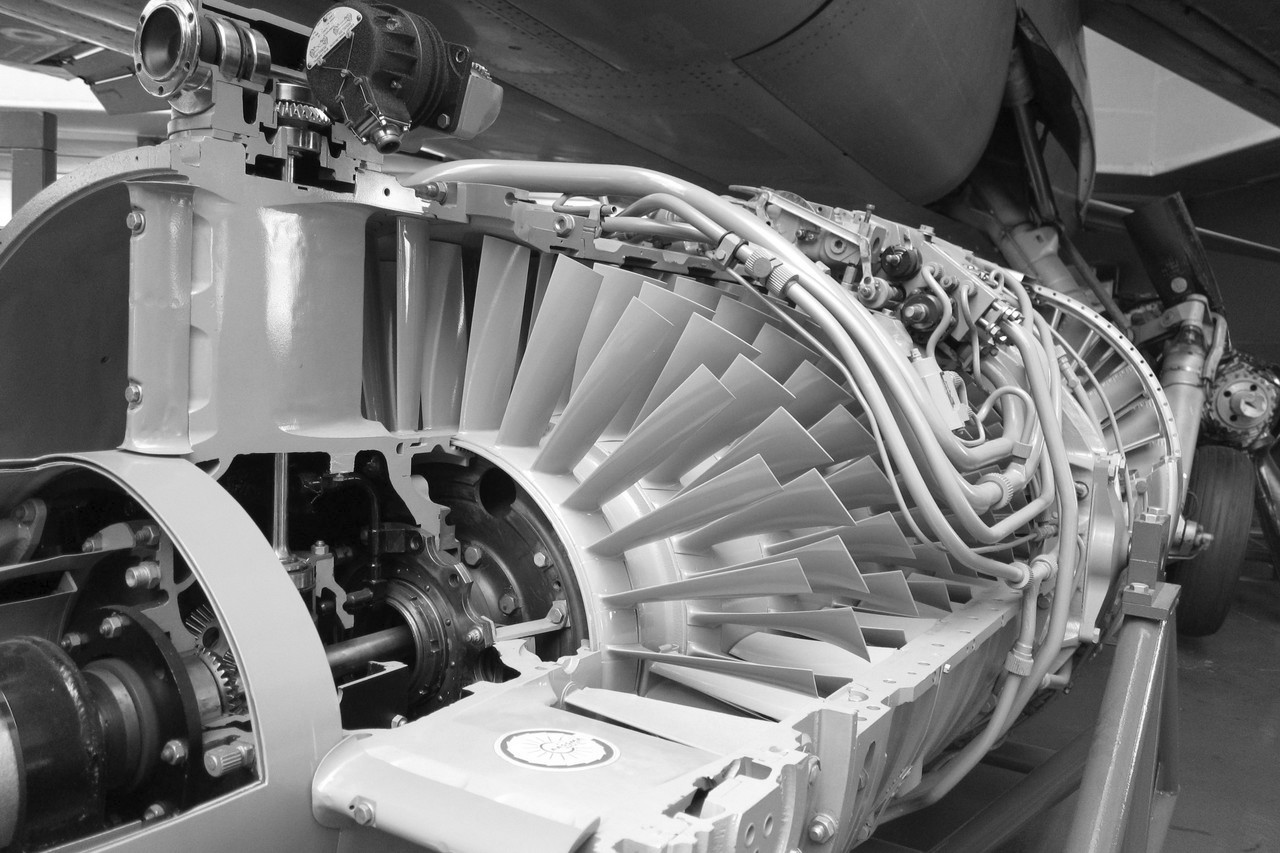
\includegraphics[width=0.8\textwidth]{images/atar_compressor.jpg}
		\end{center}
		\supercaption{Compresseur d’un turboréacteur simple flux \wfd{Snecma Atar}{\textsc{snecma} Atar} (1948) découpé. L’air s’écoule depuis le coin gauche vers le centre de l’image.}{\wcfile{Compressor of Atar turbojet.jpg}{Photo} \ccbysa \olivier}
		\label{fig_exo_compresseur_turbojet}
	\end{figure}


\exercisesolutionpage
\titreresultats

\begin{description}
	\item [\ref{exo_pression_air}]
					\tab 1) $v_1 = \frac{V_1}{m_1} = \SI{0,4}{\metre\cubed\per\kilogram}$ ; $\rho_1 = \frac{1}{v_1} = \SI{2,5}{\kilogram\per\metre\cubed}$
					\tab 2) $p_1 = \frac{R T_1}{v_1} = \SI{2,103}{\bar}$.
	\item [\ref{exo_rechauffement_reservoir_air}]
					\tab 1) $m_1 = \frac{p_1 V_1}{R T_1} = \SI{3,006}{\kilogram}$ ; $v_1 = \SI{0,3991}{\metre\cubed\per\kilogram}$ ; $\rho_1 = \SI{2,505}{\kilogram\per\metre\cubed}$ ; $p_1 = \SI{2}{\bar}$ ;
					\tab ~~ $m_2 = m_1$ ; $v_1 = v_2$ ; $\rho_1 = \rho_2$ ; $p_2 = \frac{R T_2}{v_2} = \SI{2,395}{\bar}$.\\
					\tab 2) $m_3 = \SI{2,51}{\kilogram}$, ainsi $m_\text{échap.} = m_3 - m_2 \SI{0,4959}{\kilogram}$ ;
					\tab 3) $p_4 = \frac{R T_4 m_4}{V_4} = \SI{1,67}{\bar}$.
	\item [\ref{exo_gp_energie_temperature}]
					\tab $\Delta u = c_v T_3 - u_1 = \SI{-536}{\kilo\joule\per\kilogram}$ (se calcule simplement avec la température finale et ne dépend pas de l’évolution ou des états intermédiaires).
	\item [\ref{exo_puissance_pompe_air}]
					\tab $w_{1\to 2} = \Delta h = c_p \Delta T = \SI{+85,4}{\kilo\joule\per\kilogram}$ (\ref{eq_petite_sfee_deltas_h} \& \ref{eq_h_fonction_de_T})
	\item [\ref{exo_gp_turbine_turboreacteur}]
					\tab 1) Avec l’\cref{eq_petite_sfee_deltas_h}, $w_\text{turbine} = c_p (T_\B - T_\A) + \frac{1}{2}(C_\B^2 - C_\A^2) - q_\fromatob = \SI{-275}{\kilo\joule\per\kilogram}$ 	
					\tab 2) $\dot m = \frac{\dot W_\text{turbine}}{w_\text{turbine}} = \SI{3,64}{\kilogram\per\second}$
	\item [\ref{exo_gp_isotherme}]
					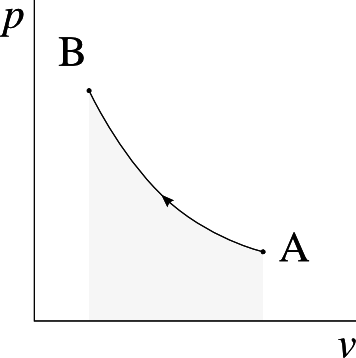
\includegraphics[width=\solutiondiagramwidth]{images/exo_sol_pv_isoth.png}
					\tab 2) Avec l’\cref{eq_gp_travail_isotherme_sf1}, $w_{1 \to 2} = \SI{+257,58}{\kilo\joule\per\kilogram}$ (donc un travail reçu) ; $W_{1 \to 2} = \SI{+901,2}{\kilo\joule}$ ; $Q_{1 \to 2} = - W_{1 \to 2}$ (donc une dépense de chaleur)\\
				 	\tab 3) Oui, on aurait $v_{2 \text{ad.rév.}} = v_1 \left(\frac{p_1}{p_2}\right)^{\frac{1}{\gamma}} > v_{2 \text{isoth.}} =  v_1 \left(\frac{p_1}{p_2}\right)$.
	\item [\ref{exo_gp_isobare_isochore}]
					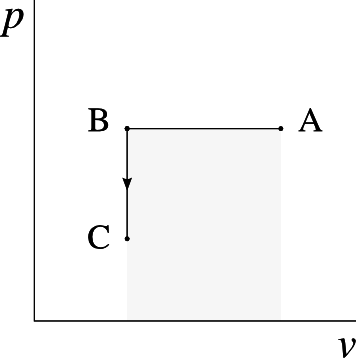
\includegraphics[width=\solutiondiagramwidth]{images/exo_sol_pv_isob_isoch.png}
					\tab 2) $W_{1 \to 3} = -\int_1^2 p \diff V - \int_2^3 p \diff V = -p_\text{cste} \Delta V - 0 = \SI{+153,6}{\kilo\joule}$	
					\tab 3) $Q_{1 \to 3} = U_3 - U_1 - W_{1 \to 3} = m c_v \left(T_3 - \frac{p_1 V_1}{m R}\right) - W_{1 \to 3} = \SI{-625,3}{\kilo\joule}$
	\item [\ref{exo_gp_isentropique}]
					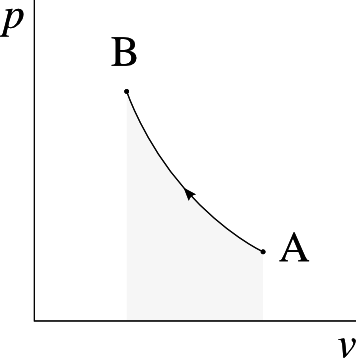
\includegraphics[width=\solutiondiagramwidth]{images/exo_sol_pv_isentr.png}
						\tab Cas optimal : compression adiabatique réversible. Avec l’équation~\ref{eq_isentropique_horrible2}, on calcule $T_\B = \SI{896,4}{\kelvin}$ ; $W_\text{minimal} = m \ c_v (T_\B - T_\A) = \SI{+2,157}{\mega\joule}$.
	\item [\ref{exo_bete_mechant}]
						\tab Isotherme $2 \to 3$, isochore $1 \to 2$.
	\item [\ref{exo_retrouver_pv}]
						\tab \textit{Dans le sens horaire, en débutant à l’horizontale, sur les deux graphiques :} isobare ($p$~cste.), isotherme ($T$~cste.), adiabatique réversible, isochore ($v$~cst.).
	\item [\ref{exo_compresseur_turboreacteur}]
						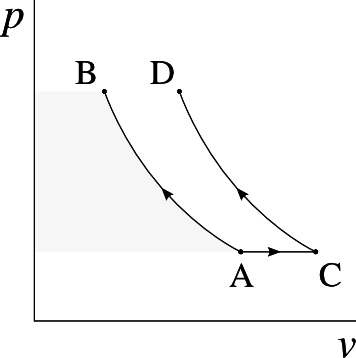
\includegraphics[width=\solutiondiagramwidth]{images/exo_sol_pv_turbojet_compressor.png}
						\tab 1) Remplacer $v_2$ par $\frac{R T_2}{p_2}$, faire de même avec $v_1$. Dérouiller son algèbre et le résultat vient tout seul ;
						\tab 2) Avec l’équation~\ref{eq_isentropique_horrible2}, on obtient $T_\B = \SI{600,7}{\kelvin}$, ainsi $\dot{W}_{\fromatob} = \SI{+20,87}{\mega\watt}$ ;
						\tab 3) \S\ref{ch_gp_isentropiques} ;
						\tab 5) $T_\C = \SI{279,8}{\kelvin}$ ; $T_\D = \SI{753,1}{\kelvin}$ ; Ainsi $\dot{W}_\text{compresseur réel} = \dot{W}_{\text{pertes frottement} \A \to \C} + \dot{W}_\fromctod = \SI{+29,29}{\mega\watt}$ (\SI{+40}{\percent}).
	\item [\ref{exo_compression_combustion_diesel}]
						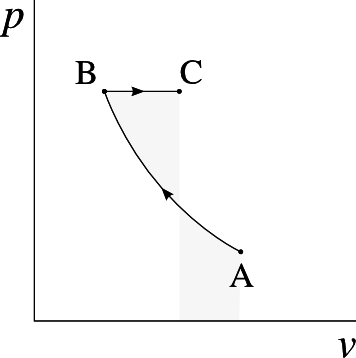
\includegraphics[width=\solutiondiagramwidth]{images/exo_sol_pv_diesel.png}
						\tab 1) voir \S\ref{ch_travail_fdl} p.\pageref{ch_travail_fdl} \& \S\ref{ch_travail_pdv} p.\pageref{ch_travail_pdv};
					 	\tab 2) $W_{\fromatob} = - m \int_\A^\B p \diff v = \SI{+1,298}{\kilo\joule}$ 	
						\tab 3) Avec $p_\B = k v_\B^{\num{-1,5}} = \SI{31,6}{\bar}$, on a $T_\B = \SI{926,3}{\kelvin}$. Enfin, $Q_{\fromatob} = \Delta U - W_{\fromatob} = \SI{+0,3254}{\kilo\joule}$.
						\tab 5) À pression constante, avec l’\cref{eq_q_gp_sf_isobare},  $T_\C = \frac{Q_\frombtoc}{m \ c_p} + T_\B = \SI{1483,7}{\kelvin}$ (\SI{1211}{\degreeCelsius}).
						\tab 6) $S < \frac{F_\text{max.}}{p_\C} = \SI{3,164e-3}{\metre\squared}$ (diamètre $D_\text{max} = \SI{6,35}{\centi\metre}$).
	\item [\ref{exo_turboreacteur_simple_flux}]
						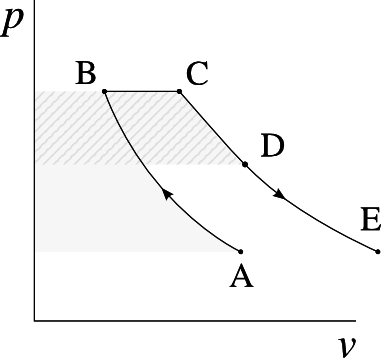
\includegraphics[width=\solutiondiagramwidth]{images/exo_sol_pv_turbojet_1.png}
						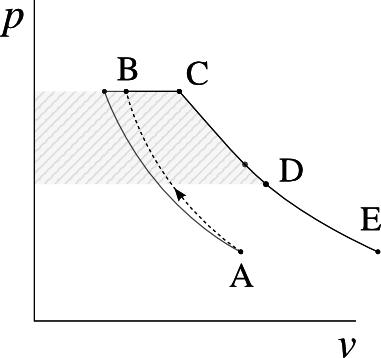
\includegraphics[width=\solutiondiagramwidth]{images/exo_sol_pv_turbojet_2.png}
						\tab 2) Avec l’équation~\ref{eq_isentropique_horrible2}, $T_\B = \SI{664,83}{\kelvin}$
						\tab 3) Avec l’\cref{eq_petite_sfee_deltas_h}, $w_\text{compresseur} = w_\fromatob = \SI{+338,61}{\kilo\joule\per\kilogram}$
						\tab 4) $T_\C = \SI{1373,15}{\kelvin}$ ; ainsi $q_\text{combustion} = q_\frombtoc = \SI{+711,86}{\kilo\joule\per\kilogram}$
						\tab 5) Comme $w_\text{turbine} = - w_\text{compresseur}$, on a $T_D = \SI{986,47}{\kelvin}$
						\tab 6) Avec l’équation~\ref{eq_isentropique_horrible2}, $p_\D = \SI{5,97}{\bar}$
						\tab 7) Idem, avec l’équation~\ref{eq_isentropique_horrible2}, $T_\text{E} = \SI{574,49}{\kelvin}$
						\tab 8) Avec l’\cref{eq_petite_sfee_deltas_h}, $C_\text{E} = \left(-2\Delta h\right)^\frac{1}{2} = \SI{909,98}{\metre\per\second}$\\
						\tab Bien sûr, ces valeurs ne tiennent pas compte des irréversibilités existant dans un turboréacteur réel. Ces effets sont abordés dans l’exercice \ref{exo_compresseur_turboreacteur} p.\pageref{exo_compresseur_turboreacteur} et formalisés dans le \coursdix.
\end{description}

\atendofexercices
